\chapter*{Programme officiel}

\section*{Programme officiel}

Le concept de méthode algorithmique est introduit ; de nouveaux exemples seront vus en terminale. Quelques algorithmes classiques sont étudiés. L'étude de leurs coûts respectifs prend tout son sens dans le cas de données nombreuses, qui peuvent être préférentiellement des données ouvertes.

Il est nécessaire de montrer l'intérêt de prouver la correction d'un algorithme pour lequel on dispose d'une spécification précise, notamment en mobilisant la notion d'invariant sur des exemples simples. La nécessité de prouver la terminaison d'un programme est mise en évidence dès qu'on utilise une boucle non bornée (ou, en terminale, des fonctions récursives) grâce à la mobilisation de la notion de variant sur des exemples simples.

{\centering\begin{tabular}{|L{3cm}|L{5.5cm}|L{6cm}|}\hline
\cellcolor{bo}\bfseries\textcolor{white}{Contenus}&
\cellcolor{bo}\bfseries\textcolor{white}{Capacités attendues}&
\cellcolor{bo}\bfseries\textcolor{white}{Commentaires}\\ \hline
Parcours séquentiel d'un tableau
&
Écrire un algorithme de recherche d'une occurrence sur des valeurs de type quelconque.

Écrire un algorithme de recherche d'un extremum, de calcul d'une moyenne.
&
On montre que le coût est linéaire.\\ \hline
Tris par insertion, par sélection
&
Écrire un algorithme de tri.

Décrire un invariant de boucle qui prouve la correction des tris par insertion, par sélection.
&
La terminaison de ces algorithmes est à justifier.

On montre que leur coût est quadratique dans le pire cas.\\ \hline
Algorithme des k plus proches voisins
&
Écrire un algorithme qui prédit la classe d'un élément en fonction de la classe majoritaire de ses k plus proches voisins.
&
Il s'agit d'un exemple d'algorithme d'apprentissage.\\ \hline
Recherche dichotomique dans un tableau trié
&
Montrer la terminaison de la recherche dichotomique à l'aide d'un variant de boucle.
&
Des assertions peuvent être utilisées.

La preuve de la correction peut être présentée par le professeur.\\ \hline
Algorithmes gloutons
&
Résoudre un problème grâce à un algorithme glouton.
&
Exemples : problèmes du sac à dos ou du rendu de monnaie.

Les algorithmes gloutons constituent une méthode algorithmique parmi d'autres qui seront vues en terminale.\\ \hline
\end{tabular}\par}


\chapter{Recherches dans un tableau}
\newcommand{\carte}[2][white]{%
\newcount\cou%
\newcount\val%
\val=#2%
\cou=#2%
\advance\cou by-1%
\divide\cou by13%
\def\couleur{$\spadesuit$}\def\couleurtexte{black}%
\ifnum\cou=1\def\couleur{$\color{rouge}\heartsuit$}\def\couleurtexte{rouge}\fi%
\ifnum\cou=2\def\couleur{$\color{rouge}\diamondsuit$}\def\couleurtexte{rouge}\fi%
\ifnum\cou=3\def\couleur{$\clubsuit$}\fi%
\multiply\cou by-13%
\advance\val by\cou%
\def\valeur{\the\val}%
\ifnum\val=11\def\valeur{V}\fi%
\ifnum\val=12\def\valeur{D}\fi%
\ifnum\val=13\def\valeur{R}\fi%
\def\dessin{\tiny\begin{tabular}{@{}c@{}}\color{\couleurtexte}\valeur\\\couleur\end{tabular}}%
\begin{tikzpicture}%
\draw[fill=#1,rounded corners=1.5pt](0,0)rectangle(1,1.5);%
\node[below right=1pt,xscale=0.75,inner sep = 0]at(0,1.5){\dessin};%
\node[below left=1pt,xscale=0.75,inner sep = 0]at(1,1.5){\dessin};%
\node[above right=1pt,xscale=0.75,inner sep = 0]at(0,0){\rotatebox{180}{\dessin}};%
\node[above left=1pt,xscale=0.75,inner sep = 0]at(1,0){\rotatebox{180}{\dessin}};%
\node[yscale=2,xscale=1.5]at(0.5,0.75){\dessin};%
\end{tikzpicture}}

\begin{center} Comment trouver une information parmi beaucoup d'autres ?

\begin{tikzpicture}
\foreach \v in {0.02,0.04,...,2.6}
\fill[opacity=0.002](4,2)ellipse(2*\v cm and \v cm);
\foreach \v/\x/\y/\a in {10	/	1.23	/	1.05	/	256	,
32	/	2.49	/	0.59	/	46	,
41	/	3.00	/	3.94	/	296	,
40	/	4.07	/	0.96	/	334	,
42	/	1.14	/	2.93	/	283	,
46	/	3.69	/	3.01	/	336	,
43	/	2.78	/	1.07	/	157	,
4	/	6.55	/	3.98	/	115	,
49	/	7.66	/	1.28	/	85	,
5	/	4.26	/	2.32	/	311	,
12	/	4.24	/	2.39	/	355	,
48	/	4.67	/	2.69	/	171	,
25	/	5.70	/	2.17	/	156	,
26	/	4.01	/	2.33	/	98	,
38	/	3.51	/	2.04	/	235	,
31	/	4.86	/	3.61	/	322	,
52	/	0.94	/	1.29	/	79	,
45	/	5.49	/	2.29	/	158	,
7	/	3.71	/	0.43	/	202	,
13	/	1.62	/	0.95	/	334	,
44	/	7.33	/	0.85	/	229	,
21	/	7.30	/	2.05	/	140	,
9	/	1.47	/	1.15	/	182	,
34	/	7.19	/	1.46	/	266	,
11	/	0.62	/	0.65	/	11	,
17	/	2.09	/	0.02	/	234	,
16	/	4.70	/	0.09	/	187	,
50	/	7.31	/	3.84	/	302	,
23	/	7.29	/	2.69	/	75	,
28	/	7.89	/	3.57	/	343	,
37	/	0.83	/	2.06	/	346	,
51	/	2.71	/	2.14	/	250	,
36	/	6.34	/	2.62	/	183	,
24	/	0.94	/	1.84	/	59	,
27	/	3.76	/	3.50	/	53	,
20	/	3.25	/	3.02	/	17	,
15	/	6.14	/	3.85	/	50	,
8	/	1.80	/	0.42	/	185	,
39	/	3.50	/	1.06	/	151	,
29	/	6.12	/	0.76	/	116	,
47	/	6.30	/	1.58	/	296	,
30	/	4.88	/	0.19	/	304	,
33	/	5.09	/	3.27	/	283	,
19	/	2.59	/	0.49	/	71	,
6	/	5.64	/	2.80	/	156	,
14	/	5.40	/	2.95	/	47	,
1	/	7.56	/	2.71	/	343	,
18	/	0.46	/	2.49	/	41	,
3	/	7.85	/	1.85	/	293	,
22	/	1.54	/	3.46	/	34	,
35	/	0.86	/	2.21	/	279	,
2	/	4.44	/	0.82	/	137	
} \node[rotate=\a]at(\x*1cm,\y*1cm){\carte{\v}};
\end{tikzpicture}\end{center}

Une solution élémentaire est de faire un tas et de passer en revue toutes les cartes une à une.

\section{Parcours séquentiel d'un tableau}

Pour simplifier l'exemple, supposons que l'on ait tiré une main et notons les valeurs des cartes dans un tableau :

\begin{center}
\begin{tikzpicture}[baseline={([yshift=-.5ex]current bounding box.center)}]
\foreach \v/\a in {25/50,1/40,33/30,52/20,29/10,31/0,24/-10,28/-20,5/-30,34/-40} 
  \draw[shift={(90+\a:0.75)},color=black]node[rotate=\a]{\carte{\v}};
\end{tikzpicture}
\begin{minipage}{8.5cm}
\begin{tabular}{|c|c|c|c|c|c|c|c|c|c|}
\hline
\small DC &\small 1P &\small 7c &\small RT &\small 3c &\small 5c&\small VC&\small 2c&\small 5P&\small 8c\\
\hline
\end{tabular}
\end{minipage}

\pythoninline{ cartes = ['DC', '1P', '7c', 'RT', '3c', '5c', 'VC', '2c', '5P', '8c']}
\end{center}

\subsection{Spécification possible}

\begin{itemize}
	\item {\bfseries Entrée :} Tableau $T$ de longueur $n$, et une valeur $v$.
	\item {\bfseries Sortie :} Un indice $i$ de $v$ dans $T$ ou $-1$ si $v$ n'est pas dans $T$. 
	\item {\bfseries Rôle :} Recherche d'une occurrence de $v$ dans $T$.
	\item {\bfseries Précondition :} $v$ est comparable avec les éléments de $T$.
	\item {\bfseries Postcondition :} ($i=-1$ et $v$ n'est pas dans $T$) ou ($0\leqslant i < n$ et $T[i]$ est $v$).
\end{itemize}

\subsection{Algorithme}

\begin{algorithm}[H]
$i \leftarrow -1$\;
\Pour{$carte$ {\normalfont\bfseries allant de} $0$ {\normalfont\bfseries à} $n-1$}
{ \Si{$\text{\normalfont T}[carte]==v$}
  {  $i\leftarrow carte$\;  }
}
\end{algorithm}

\subsection{Correction et complexité}

\begin{itemize}
	\item {\bfseries Correction partielle :} On peut prendre comme invariant, pour la boucle \texttt{pour}, la postcondition limitée au sous-tableau déjà parcouru.
	
	Invariant : ($i=-1$ et si $0\leqslant j\leqslant carte$ alors $\text{\normalfont T}[j]\ne v$) ou ($0\leqslant i \leqslant carte$ et $\text{\normalfont T}[i]=v$).
	
	Avant la première itération $carte$ n'est pas définie et on a bien $i=-1$.
	
	Après la première itération $carte=0$ ; si la condition $\text{\normalfont T}[carte]==v$ a été vérifiée, alors on a $0= i = carte$ donc $0\leqslant i \leqslant carte$ et $\text{\normalfont T}[i]=v$ ; sinon, on a toujours $ i = -1$ et pour $0\leqslant j\leqslant carte$ c'est à dire $j=0$, on a aussi  $\text{\normalfont T}[j]\ne v$. L'invariant est donc vérifié.
	
	S'il est vérifié avant une itération, alors on peut distinguer 4 cas :
	\begin{itemize}
		\item ($i=-1$ et si $0\leqslant j\leqslant carte$ alors $\text{\normalfont T}[j]\ne v$) et la conditionnelle se réalise ;
		\item ($i=-1$ et si $0\leqslant j\leqslant carte$ alors $\text{\normalfont T}[j]\ne v$) et la conditionnelle ne se réalise pas ;
		\item ($0\leqslant i \leqslant carte$ et $\text{\normalfont T}[i]=v$)  et la conditionnelle se réalise ;
		\item ($0\leqslant i \leqslant carte$ et $\text{\normalfont T}[i]=v$)  et la conditionnelle ne se réalise pas.
	\end{itemize}
	
	Dans chaque cas, on peut vérifier comme précédemment que l'invariant est bien conservé.
	
	Enfin, l'expression de l'invariant après la dernière itération donne la postcondition.
	\item {\bfseries Terminaison :} Une boucle \texttt{pour} termine.
	\item {\bfseries Complexité :} La taille des entrées est la longueur $n$ du tableau.
	
	Le pire cas vient d'une réalisation systématique de la condition $\text{\normalfont T}[carte]=v$, c'est à dire un tableau dont toutes les valeurs sont égales à $v$.
	
	Dans ce cas, on peut compter 3 opérations par itération (mise à jour de $carte$, comparaison de la conditionnelle, et affectation de $i$). La boucle faisant $n$ itérations, on obtient en tout $3n+1$ opérations.
	
	$3n+1 = O(n)$. La complexité est linéaire.
\end{itemize}

\subsection{Applications}

Appliquons l'algorithme précédent à un tableau de nombres :

\pythoninline{tableau = [1, 5, 7, 3, 2, 9, 4, 6]}

\subsubsection{Recherche d'un maximum}

La valeur recherchée n'est pas connue, mais vérifie un critère. 

Ajoutons la {\bfseries précondition} suivante pour initialiser : $T$ n'est pas vide.

On peut alors adapter l'algorithme précédent :

\begin{algorithm}[H]
$max \leftarrow T[0]$\;
\Pour{$i$ {\normalfont\bfseries allant de} $0$ {\normalfont\bfseries à} $n-1$}
{ \Si{$\text{\normalfont T}[i]>max$}
  {  $max \leftarrow \text{\normalfont T}[i]$\;  }
}
\end{algorithm}

Une preuve similaire s'applique et la complexité est toujours linéaire.


\subsubsection{Calcul d'une moyenne}

Toutes les valeurs sont utilisées : l'algorithme est simplifié (plus de conditionnelle).

\begin{algorithm}[H]
$somme \leftarrow 0$\;
\Pour{$i$ {\normalfont\bfseries allant de} $0$ {\normalfont\bfseries à} $n-1$}
{ $somme \leftarrow somme + \text{\normalfont T}[i]$\;  }
$moyenne \leftarrow somme / n$\;
\end{algorithm}

Un invariant possible pour la correction partielle : $somme$ est la somme des valeurs de T d'indices inférieurs à $i$.

La complexité est toujours linéaire.


\section{Recherche dichotomique}

On rajoute ici une précondition importante : Le tableau est \emph{trié}.

On pourrait définir plusieurs critères (couleur / valeur / points dans un jeu ...). Dans ce qui suit, on supposera établi un ordre total qui permet la numérotation :

\begin{center}\begin{tikzpicture}
\foreach \v in {1,...,52} {
  \node at(\v*0.28cm,0cm){\carte{\v}};
  \node[scale=0.6,xshift=-0.7cm,yshift=-1.3cm,below]at(\v*0.28cm,0){\v};
 }
\end{tikzpicture}
\end{center}

On peut réécrire notre main :

\vspace{-3ex}
\begin{center}\begin{tikzpicture}[baseline={([yshift=-.5ex]current bounding box.center)}]
\foreach \v/\a in {25/50,1/40,33/30,52/20,29/10,31/0,24/-10,28/-20,5/-30,34/-40} 
  \draw[shift={(90+\a:0.75)},color=black]node[rotate=\a]{\carte{\v}};
\end{tikzpicture}
\begin{minipage}{8.5cm}
\begin{tabular}{|c|c|c|c|c|c|c|c|c|c|}
\hline
\small 25&\small 1&\small 33&\small 52&\small 29&\small 31&\small 24&\small 28&\small 5&\small 34\\
\hline
\end{tabular}
\medskip

\pythoninline{ cartes = [25,1,33,52,29,31,24,28,5,34]}
\end{minipage}\end{center}

Et la trier :

\vspace{-4ex}
\begin{center}\begin{tikzpicture}[baseline={([yshift=-.5ex]current bounding box.center)}]
\foreach \v/\a in {1/50,5/40,24/30,25/20,28/10,29/0,31/-10,33/-20,34/-30,52/-40} 
  \draw[shift={(90+\a:0.75)},color=black]node[rotate=\a]{\carte{\v}};
\end{tikzpicture}
\begin{minipage}{8.5cm}
\begin{tabular}{|c|c|c|c|c|c|c|c|c|c|}
\hline
\small 1&\small 5&\small 24&\small 25&\small 28&\small 29&\small 31&\small 33&\small 34&\small 52\\
\hline
\end{tabular}
\medskip

\pythoninline{ cartes = [1,5,24,25,28,29,31,33,34,52]}
\end{minipage}\end{center}

On ajoute à la {\bfseries précondition :} $T$ est non vide et trié.


\subsection{Algorithme}

Une recherche \emph{dichotomique} consiste, par comparaison, à éliminer au moins la moitié des possibilités à chaque étape. L'idée est donc de faire ces comparaisons avec des médianes parmi des valeurs triées. 

Sur l'exemple, cherchons le cinq de carreau (le 31). Pour la médiane du sous tableau entre les indices $min$ et $max$, on choisit la valeur d'indice $(min+max)//2$ :

\begin{center}

\begin{minipage}{9.5cm}\begin{center}
\begin{tikzpicture}
\foreach \v/\a in {1/50,5/40,24/30,25/20}  
  \draw[shift={(90+\a:0.75)},color=black]node[rotate=\a]{\carte{\v}};
\foreach \v/\a in {28/10} 
  \draw[shift={(90+\a:0.85)},color=black]node[rotate=\a]{\carte[black!30]{\v}};
\foreach \v/\a in {29/0,31/-10,33/-20,34/-30,52/-40}  
  \draw[shift={(90+\a:0.75)},color=black]node[rotate=\a]{\carte{\v}};
\end{tikzpicture}
\begin{tikzpicture}
\foreach \v/\a in {29/0,31/-10}  
  \draw[shift={(90+\a:0.75)},color=black]node[rotate=\a]{\carte{\v}};
\foreach \v/\a in {33/-20} 
  \draw[shift={(90+\a:0.85)},color=black]node[rotate=\a]{\carte[black!30]{\v}};
\foreach \v/\a in {34/-30,52/-40}  
  \draw[shift={(90+\a:0.75)},color=black]node[rotate=\a]{\carte{\v}};
\end{tikzpicture}
\begin{tikzpicture}
\foreach \v/\a in {29/0} 
  \draw[shift={(90+\a:0.85)},color=black]node[rotate=\a]{\carte[black!30]{\v}};
\foreach \v/\a in {31/-10}  
  \draw[shift={(90+\a:0.75)},color=black]node[rotate=\a]{\carte{\v}};
\end{tikzpicture}
\begin{tikzpicture}
\foreach \v/\a in {31/-10} 
  \draw[shift={(90+\a:0.85)},color=black]node[rotate=\a]{\carte[black!30]{\v}};
\end{tikzpicture}

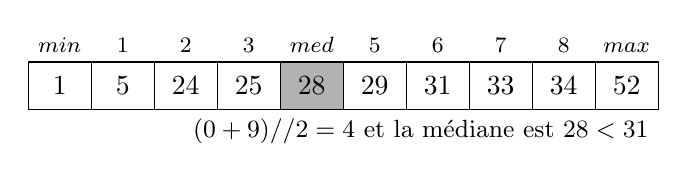
\begin{tikzpicture}
\foreach \a in {-10}
  \fill[xshift=0.08cm*\a,color=black!30](6.1,0.2)rectangle(6.9,0.8);
\foreach \i/\v in {0/min,1/1,2/2,3/3,4/med,5/5,6/6,7/7,8/8,9/max} \node[above]at(2.5cm+\i*0.8cm,0.8){\footnotesize $\v$};
\node[below left]at(2.9cm+9*0.8cm,0.2){\small $(0+9)//2=4$ et la médiane est $28<31$};
\foreach \v/\a in {1/50,5/40,24/30,25/20,28/10,29/0,31/-10,33/-20,34/-30,52/-40}  {
  \node[xshift=-0.08cm*\a]at(6.5,0.5){\v};
  \draw[xshift=-0.08cm*\a](6.1,0.2)rectangle(6.9,0.8);
}
\end{tikzpicture}

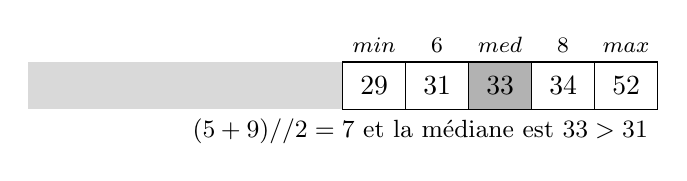
\begin{tikzpicture}
\foreach \a in {-50,-40,...,-10}
  \fill[xshift=0.08cm*\a,color=black!15](6.1,0.2)rectangle(6.9,0.8);
\foreach \a in {20}
  \fill[xshift=0.08cm*\a,color=black!30](6.1,0.2)rectangle(6.9,0.8);
\foreach \i/\v in {5/min,6/6,7/med,8/8,9/max} \node[above]at(2.5cm+\i*0.8cm,0.8){\footnotesize $\v$};
\node[below left]at(2.9cm+9*0.8cm,0.2){\small $(5+9)//2=7$ et la médiane est $33>31$};
\foreach \v/\a in {29/0,31/-10,33/-20,34/-30,52/-40}  {
  \node[xshift=-0.08cm*\a]at(6.5,0.5){\v};
  \draw[xshift=-0.08cm*\a](6.1,0.2)rectangle(6.9,0.8);
}
\end{tikzpicture}

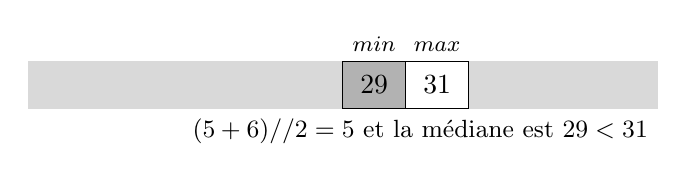
\begin{tikzpicture}[baseline={([yshift=-.5ex]current bounding box.center)}]
\foreach \a in {-50,-40,...,-10,20,30,40}
  \fill[xshift=0.08cm*\a,color=black!15](6.1,0.2)rectangle(6.9,0.8);
\foreach \a in {0}
  \fill[xshift=0.08cm*\a,color=black!30](6.1,0.2)rectangle(6.9,0.8);
\foreach \i/\v in {5/min,6/max} \node[above]at(2.5cm+\i*0.8cm,0.8){\footnotesize $\v$};
\node[below left]at(2.9cm+9*0.8cm,0.2){\small $(5+6)//2=5$ et la médiane est $29<31$};
\foreach \v/\a in {29/0,31/-10}  {
  \node[xshift=-0.08cm*\a]at(6.5,0.5){\v};
  \draw[xshift=-0.08cm*\a](6.1,0.2)rectangle(6.9,0.8);
}
\end{tikzpicture}


\begin{tikzpicture}[baseline={([yshift=-.5ex]current bounding box.center)}]
\foreach \a in {-50,-40,...,0,20,30,40}
  \fill[xshift=0.08cm*\a,color=black!15](6.1,0.2)rectangle(6.9,0.8);
\foreach \a in {10}
  \fill[xshift=0.08cm*\a,color=black!30](6.1,0.2)rectangle(6.9,0.8);
\foreach \i in {6} \node[above]at(2.5cm+\i*0.8cm,0.8){\footnotesize $min = max$};
\foreach \v/\a in {31/-10}  {
  \node[xshift=-0.08cm*\a]at(6.5,0.5){\v};
  \draw[xshift=-0.08cm*\a](6.1,0.2)rectangle(6.9,0.8);
}
\end{tikzpicture}\end{center}
\end{minipage}\begin{minipage}{6.5cm}\begin{algorithm}[H]
$min \leftarrow 0$\;
$med \leftarrow 0$\;
$max \leftarrow n-1$\;
\Tq{$min < max$}
{ $med\leftarrow (min+max)//2$\;
  \uSi {$T[med] < v$}{$min\leftarrow med+1$}
  \uSinonSi {$T[med] > v$}{$max\leftarrow med-1$}
  \Sinon { $max\leftarrow med$\; $min\leftarrow med$\;}
}
\eSi{$T[min] = v$}{$i \leftarrow min$}{$i \leftarrow -1$\;}
\end{algorithm}\end{minipage}
\end{center}


\subsection{Correction}

\begin{itemize}
	\item {\bfseries Correction partielle} 
	
	Montrons l'invariant : << $T[min] \leqslant v \leqslant T[max]$ ou $v$ n'est pas dans le tableau >>.
	
	Il est vrai au début de la boucle puisque tout le tableau est entre $min$ et $max$.
	
	Supposons-le vrai au début d'une itération.
	
	Comme on ne modifie jamais le tableau, si $v$ n'est pas dans le tableau, il n'y sera jamais.
	
	On va donc supposer que $v$ est dans le tableau.
	
	\begin{itemize}
		\item Comme $min < max$, le calcul (ligne 6) de $med$ donne : $min \leqslant med < max$.
		\item Cas du passage ligne 7 : 
		
		Comme le tableau est trié,  avant l'exécution : $T[min] \leqslant T[med] < v \leqslant T[max]$
		
		Si on avait $T[med+1] > v$ alors on aurait $T[med]< v <T[med+1]$ et $v$ ne serait pas dans le tableau, donc $T[med+1] \leqslant v \leqslant T[max]$ et la ligne 7 conserve l'invariant.
		\item Cas du passage ligne 9 : 
		
		Comme le tableau est trié,  avant l'exécution : $T[min] \leqslant v < T[med]  \leqslant T[max]$
		
		Si on avait $T[med-1] < v$ alors on aurait $T[med-1]< v <T[med]$ et $v$ ne serait pas dans le tableau, donc $T[min] \leqslant v \leqslant T[med-1]$ et la ligne 9 conserve l'invariant.
		
		\item Cas du passage lignes 11 et 12 : 
		
		En excluant les deux inégalités précédentes, il ne reste que  $T[med] = v$
		
		Les lignes 11 et 12 conservent donc l'invariant.
		
		
		\item L'invariant est donc bien toujours vérifié.
	\end{itemize}
	
	Si on sort de la boucle : $min \geqslant max$ donc $T[min] \geqslant T[max]$.
	
	L'invariant donne alors << $T[min] = v = T[max]$ ou $v$ n'est pas dans le tableau >>
	
	Donc $v$ est dans le tableau si et seulement si $T[min] = v$.
	
	
	\item {\bfseries Terminaison :}
	
	L'expression $max - min$ est minorée par la condition de la boucle à 0.
	
	Si on ne passe jamais par les lignes 11 et 12, $max - min$ est strictement décroissante.
	
	Dans ce cas on a bien un variant qui permet d'assurer que l'algorithme termine.
	
	Si on passe par les lignes 11 et 12 alors $max - min$ devient 0 et l'algorithme termine.
\end{itemize}

\subsection{Complexité}

La taille des entrées est la longueur $n$ du tableau.

Comme on élimine à chaque itération au moins la moitié des valeurs du tableau, si on peut déterminer pour quel entier $N$ on a $2^{N-1} < n \leqslant 2^N$, et si on note $n_k$ la longueur du tableau restant après $k$ itérations :

$n_0 = n \leqslant 2^N$ puis $n_1 \leqslant \frac{n}{2} \leqslant 2^{N-1}$ puis $n_2 \leqslant 2^{N-2}$ ... puis $n_N \leqslant 2^{N-N} = 1$.

Donc il faut au plus $N$ itérations.

\medskip

Il existe une fonction mathématique : $\text{log}_2()$ qui donne le réel vérifiant $n = 2 ^{\text{log}_2(n)}$. On peut donc majorer le nombre d'itérations par l'entier directement supérieur à $\text{log}_2(n)$.

On dit que la complexité est logarithmique et on la note simplement : $O(\text{log}(n))$



\chapter{Tris de tableaux}

A l'ère de l'open data, la difficulté n'est plus guère de trouver de l'information mais de trier les informations disponibles pour réellement trouver celles que l'on cherche. Il existe de nombreux algorithmes de tri, certains très généraux et d'autres plus spécifiques selon les préconditions du problème. Donnons une spécification générale et traitons de deux exemples : le tri par insertion et le tri par sélection.

\medskip

{\bfseries Spécification :} 


\begin{itemize}
	\item {\bfseries Entrée / Sortie :} Tableau $T$ de longueur $n$.
	\item {\bfseries Rôle :} Trier les valeur dans $T$ par ordre croissant.
	\item {\bfseries Précondition :} Les valeurs de $T$ sont toutes comparables.
	\item {\bfseries Postcondition :} Si $0 \leqslant i\leqslant j \leqslant n-1$ alors $T[i]\leqslant T[j]$.
	
	Et les valeurs de $T$ sont les mêmes (dans un autre ordre) en entrée et en sortie.
\end{itemize}

\section{Tri par insertion}

\subsection{Algorithme}

C'est un des tris les plus simples. On prend une carte à la fois dans l'ordre de la main (de gauche à droite) et on l'insère à sa place parmi les cartes que l'on a déjà rangées (à gauche).

\begin{center}
\begin{minipage}{12.5cm}
\vspace{-0.3cm}
\noindent{\flushright
\begin{tikzpicture}[baseline={([yshift=-.5ex]current bounding box.center)}]
\def\a{-40}
\fill[xshift=0.08cm*\a,color=black!30](6.1,0.2)rectangle(6.9,0.8);
\foreach \v/\a in {25/50,1/40,33/30,52/20,29/10,31/0,24/-10,28/-20,5/-30,34/-40}  {
  \draw[shift={(90+\a:0.75)},color=black]node[rotate=\a]{\carte{\v}};
  \node[xshift=-0.08cm*\a]at(6.5,0.5){\v};
  \draw[xshift=-0.08cm*\a](6.1,0.2)rectangle(6.9,0.8);
}
\draw[-latex](3.3,0.8)to[out=90,in=90](2.5,0.8);
\draw[-latex](2.5,0.2)to[out=-90,in=-90](3.3,0.2);
%
\draw[-latex](-1.25,1)|-(-1.4,1.5)node[above]{\footnotesize insertion}-|(-1.4,0.8);
\end{tikzpicture}

\vspace{-0.5cm}
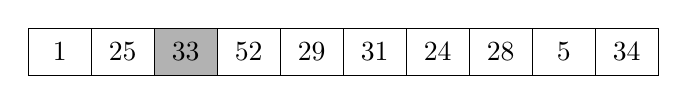
\begin{tikzpicture}[baseline={([yshift=-.5ex]current bounding box.center)}]
\def\a{-30}
\fill[xshift=0.08cm*\a,color=black!30](6.1,0.2)rectangle(6.9,0.8);
\foreach \v/\a in {1/50,25/40,33/30,52/20,29/10,31/0,24/-10,28/-20,5/-30,34/-40}  {
  \node[xshift=-0.08cm*\a]at(6.5,0.5){\v};
  \draw[xshift=-0.08cm*\a](6.1,0.2)rectangle(6.9,0.8);
}
\end{tikzpicture}

\vspace{0.2cm}
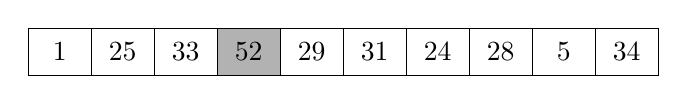
\begin{tikzpicture}[baseline={([yshift=-.5ex]current bounding box.center)}]
\def\a{-20}
\fill[xshift=0.08cm*\a,color=black!30](6.1,0.2)rectangle(6.9,0.8);
\foreach \v/\a in {1/50,25/40,33/30,52/20,29/10,31/0,24/-10,28/-20,5/-30,34/-40}  {
  \node[xshift=-0.08cm*\a]at(6.5,0.5){\v};
  \draw[xshift=-0.08cm*\a](6.1,0.2)rectangle(6.9,0.8);
}
\end{tikzpicture}

\vspace{-0.95cm}
\begin{tikzpicture}[baseline={([yshift=-.5ex]current bounding box.center)}]
\def\a{-10}
\fill[xshift=0.08cm*\a,color=black!30](6.1,0.2)rectangle(6.9,0.8);
\foreach \v/\a in {1/50,25/40,33/30,52/20,29/10,31/0,24/-10,28/-20,5/-30,34/-40}  {
  \draw[shift={(90+\a:0.75)},color=black]node[rotate=\a]{\carte{\v}};
  \node[xshift=-0.08cm*\a]at(6.5,0.5){\v};
  \draw[xshift=-0.08cm*\a](6.1,0.2)rectangle(6.9,0.8);
}
\draw[-latex](5.7,0.8)to[out=90,in=90, looseness=0.4](4.1,0.8);
\draw[-latex,xshift=0.8*2cm](2.5,0.2)to[out=-90,in=-90](3.3,0.2);
\draw[-latex,xshift=0.8*3cm](2.5,0.2)to[out=-90,in=-90](3.3,0.2);
%
\draw[-latex](-0.66,1.45)|-(-1.24,1.5)node[above]{\footnotesize insertion}-|(-1.24,1);
\end{tikzpicture}

\vspace{-0.5cm}
etc...
\par}\end{minipage}

\begin{algorithm}[H]
\Pour{$i$ {\normalfont\bfseries allant de} $1$ {\normalfont\bfseries à} $n-1$}
{ $\text{insert}\leftarrow\text{Tableau}[i]$\;
  $j\leftarrow i$\;
  \Tq {$j>0$ et $\text{\normalfont Tableau}[j-1]>\text{\normalfont insert}$}
  {   $\text{Tableau}[j]\leftarrow\text{Tableau}[j-1]$\;
      $j\leftarrow j-1$\;
  }
  $\text{Tableau}[j]\leftarrow\text{insert}$\;
}
\end{algorithm}
\end{center}

\subsection{Correction}

\subsubsection{Correction partielle}

Reformulons la première postcondition ($0 \leqslant p\leqslant k \leqslant n-1 \Rightarrow T[p]\leqslant T[k]$).

Un invariant de la boucle \texttt{pour} serait : ($0 \leqslant p\leqslant k \leqslant i \Rightarrow T[p]\leqslant T[k]$).

Si le tableau est vide, il ne se passe rien. S'il ne contient qu'un élément, l'invariant est vrai pour $i=0$ car il ne concerne qu'un élément et il ne se passe rien d'autre. Supposons donc qu'il soit vrai avant le début d'une itération, pour $i\geqslant0$, et démontrons le, après l'itération, pour $i'=i+1$.



On a donc ($0 \leqslant p\leqslant k \leqslant i \Rightarrow T[p]\leqslant T[k]$).

Ligne 2, on mémorise  $T[i']$ dans la variable insert

Si $T[i']>T[i]$, la boucle \texttt{tant que} ne fait rien, donc les lignes 3 et 7 non plus, et l'invariant est vérifié.

Sinon, dès la première ligne de la boucle \texttt{tant que}, $T[i']\leftarrow T[i]$ donc l'invariant est vérifié, et chaque autre itération de cette boucle conserve l'invariant.

A la sortie, toutes les valeurs d'indice supérieur à $j$ sont plus grandes que insert et les autres plus petites, donc la ligne 7 conserve l'invariant.

\medskip

Pour la seconde postcondition, on peut constater qu'à chaque itération, en incluant la variable insert, aucune valeur du tableau n'est perdue, car on affecte uniquement sur des doublons. De plus, la dernière affectation provoque un doublon de la variable insert dans le tableau. Donc la seconde postcondition est un invariant de la boucle \texttt{pour}. 

\subsubsection{Terminaison}

Une boucle \texttt{pour} termine toujours.

Pour la boucle \texttt{tant que} le variant est simplement \texttt{j} qui décroit strictement (de 1 à chaque itération) et est minoré par 0 (condition de la boucle).

Donc cet algorithme termine.


\subsection{Complexité}

\begin{itemize}
	\item La taille des données à traiter est la taille $n$ du tableau.
	\item L'opération significative est la modification du tableau : $\text{Tableau}[i]\leftarrow...$
	\item Cette opération apparaît directement une fois dans la boucle \texttt{pour} donc $n-1$ fois.
	
	Elle apparaît également une fois dans la boucle \texttt{tant que}:
	
	\begin{itemize}
		\item Le pire cas est donc celui qui retarde au maximum la sortie de cette boucle, c'est à dire quand toutes les valeurs déjà triées sont plus grandes que la suivante.
		
		{\centering Pire cas : Tableau trié à l'envers.}
		\item Dans ce cas il y a $i$ affectations dans le tableau.
		\item Au total il y en a donc $1+2+3+\ldots+(n-1)$.
	\end{itemize}
	
	Chacun des $(n-1)$ termes de cette somme est inférieur à $n$.
	
	On peut donc la majorer : $1+2+3+\ldots+(n-1) \leqslant n+n+n+\ldots+n = n(n-1)=O(n^2)$.
	
	(Un peu de mathématiques montre qu'elle vaut $\frac{n(n-1)}{2}$ mais toujours $O(n^2)$.)
	
	\item Bilan : $n-1+O(n^2) = O(n^2)$. La  complexité est quadratique.
\end{itemize} 



\section{Tri par sélection}

\subsection{Algorithme}

Le tri par sélection consiste à sélectionner la carte que l'on souhaite ranger au lieu de prendre la première venue. Les cartes sont choisies de la plus petite à la plus grande et positionnées directement à leurs places définitives (par échange, sans décalage).

\vspace{-0.3cm}
\noindent{\center
\begin{tikzpicture}[baseline={([yshift=-.5ex]current bounding box.center)}]
\foreach \v/\a in {25/50}  {
  \draw[shift={(90+\a:0.75)},color=black]node[rotate=\a]{\carte{\v}};
}
\foreach \v/\a in {1/40}  {
  \draw[shift={(90+\a:0.85)},color=black]node[rotate=\a]{\carte[black!30]{\v}};
}
\foreach \v/\a in {33/30,52/20,29/10,31/0,24/-10,28/-20,5/-30,34/-40}  {
  \draw[shift={(90+\a:0.75)},color=black]node[rotate=\a]{\carte{\v}};
}
\draw[|-latex](-1.25,1.1)--(-1.25,1.8)node[above]{\footnotesize sélection}-|(-1.4,0.7);
\end{tikzpicture}
\begin{tikzpicture}[baseline={([yshift=-.5ex]current bounding box.center)}]
\foreach \v/\a in {1/50}  {
  \draw[shift={(90+\a:0.75)},color=black]node[rotate=\a]{\carte[black!15]{\v}};
}
\foreach \v/\a in {25/40,33/30,52/20,29/10,31/0,24/-10,28/-20}  {
  \draw[shift={(90+\a:0.75)},color=black]node[rotate=\a]{\carte{\v}};
}
\foreach \v/\a in {5/-30}  {
  \draw[shift={(90+\a:0.85)},color=black]node[rotate=\a]{\carte[black!30]{\v}};
}
\foreach \v/\a in {34/-40}  {
  \draw[shift={(90+\a:0.75)},color=black]node[rotate=\a]{\carte{\v}};
}
\draw[|-latex](0.4,1.65)--(0.4,1.8)node[above]{\footnotesize sélection}-|(-1.24,1);
\end{tikzpicture}
\begin{tikzpicture}[baseline={([yshift=-.5ex]current bounding box.center)}]
\foreach \v/\a in {1/50,5/40}  {
  \draw[shift={(90+\a:0.75)},color=black]node[rotate=\a]{\carte[black!15]{\v}};
}
\foreach \v/\a in {33/30,52/20,29/10,31/0}  {
  \draw[shift={(90+\a:0.75)},color=black]node[rotate=\a]{\carte{\v}};
}
\foreach \v/\a in {24/-10}  {
  \draw[shift={(90+\a:0.85)},color=black]node[rotate=\a]{\carte[black!30]{\v}};
}
\foreach \v/\a in {28/-20,25/-30,34/-40}  {
  \draw[shift={(90+\a:0.75)},color=black]node[rotate=\a]{\carte{\v}};
}
\draw[|-latex](-0.1,1.7)--(-0.1,1.8)node[above]{\footnotesize sélection}-|(-1.08,1.2);
\end{tikzpicture}
etc.\par
}

\vspace{-2em}
\begin{center}\begin{minipage}{11.5cm}{\flushright
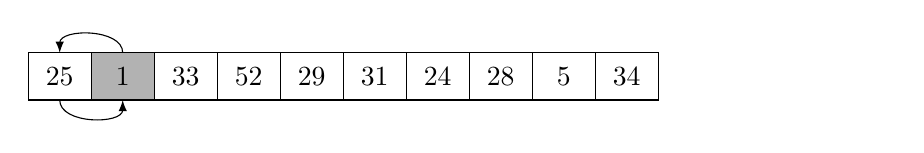
\begin{tikzpicture}[baseline={([yshift=-.5ex]current bounding box.center)}]
\def\a{-40}
\fill[xshift=0.08cm*\a,color=black!30](6.1,0.2)rectangle(6.9,0.8);
\foreach \v/\a in {25/50,1/40,33/30,52/20,29/10,31/0,24/-10,28/-20,5/-30,34/-40}  {
  \node[xshift=-0.08cm*\a]at(6.5,0.5){\v};
  \draw[xshift=-0.08cm*\a](6.1,0.2)rectangle(6.9,0.8);
}
\draw[-latex](3.3,0.8)to[out=90,in=90](2.5,0.8);
\draw[-latex](2.5,0.2)to[out=-90,in=-90](3.3,0.2);
\node at(13,0){};
\end{tikzpicture}

\vspace{-0.1cm}
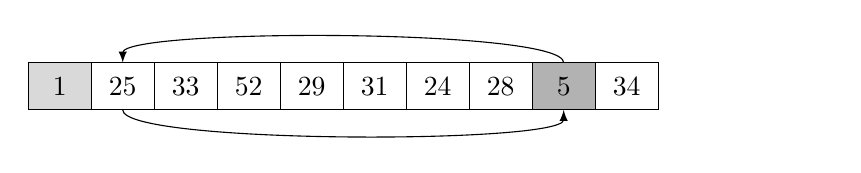
\begin{tikzpicture}[baseline={([yshift=-.5ex]current bounding box.center)}]
\def\a{30}
\fill[xshift=0.08cm*\a,color=black!30](6.1,0.2)rectangle(6.9,0.8);
\def\a{-50}
\fill[xshift=0.08cm*\a,color=black!15](6.1,0.2)rectangle(6.9,0.8);
\foreach \v/\a in {1/50,25/40,33/30,52/20,29/10,31/0,24/-10,28/-20,5/-30,34/-40}  {
  \node[xshift=-0.08cm*\a]at(6.5,0.5){\v};
  \draw[xshift=-0.08cm*\a](6.1,0.2)rectangle(6.9,0.8);
}
\draw[-latex](8.9,0.8)to[out=90,in=90, looseness=0.2](3.3,0.8);
\draw[-latex](3.3,0.2)to[out=-90,in=-90, looseness=0.2](8.9,0.2);
\node at(12.2,0){};
\end{tikzpicture}

\vspace{-0.1cm}
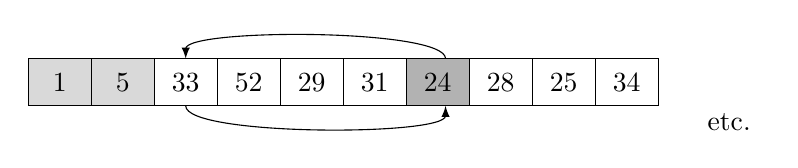
\begin{tikzpicture}[baseline={([yshift=-.5ex]current bounding box.center)}]
\def\a{10}
\fill[xshift=0.08cm*\a,color=black!30](6.1,0.2)rectangle(6.9,0.8);
\foreach \a in {-50,-40}
\fill[xshift=0.08cm*\a,color=black!15](6.1,0.2)rectangle(6.9,0.8);
\foreach \v/\a in {1/50,5/40,33/30,52/20,29/10,31/0,24/-10,28/-20,25/-30,34/-40}  {
  \node[xshift=-0.08cm*\a]at(6.5,0.5){\v};
  \draw[xshift=-0.08cm*\a](6.1,0.2)rectangle(6.9,0.8);
}
\draw[-latex](7.4,0.8)to[out=90,in=90, looseness=0.3](4.1,0.8);
\draw[-latex](4.1,0.2)to[out=-90,in=-90, looseness=0.3](7.4,0.2);
\node at(11.4,0){};
\node[left] at(11.4,0){etc.};
\end{tikzpicture}\par}
\end{minipage}

\begin{algorithm}[H]
\Pour{$i$ {\normalfont\bfseries allant de} $0$ {\normalfont\bfseries à} $\text{tailleTableau}-1$}
{ 
  $imin\leftarrow i$\;
  \Pour{$j$ {\normalfont\bfseries allant de} $i+1$ {\normalfont\bfseries à} $\text{tailleTableau}-1$}
  { \Si {$T[imin]> T[j]$}
     {$imin\leftarrow j$\;}
  }
  $T[imin], T[i] \leftarrow T[i], T[imin]$\;
}
\end{algorithm}
\end{center}


\subsection{Preuve de correction}

\subsubsection{Correction partielle}

Les éléments du tableau ne changent pas : on ne fait que des permutations simples.

Pour l'autre partie de la postcondition, on peut montrer que jusqu'à $i$ le tableau est trié et que tous les éléments suivants sont plus grands.

L'invariant : ($0 \leqslant p \leqslant k \leqslant i < m \leqslant n-1 \Rightarrow T[p]\leqslant T[k]\leqslant T[m]$).

On a déjà discuté de la recherche d'extremum. C'est ce que fait la boucle \texttt{pour j}

La boucle \texttt{pour i} se contente donc de mettre en $i$ la plus petite valeur parmi celles d'indice supérieur. On peut donc vérifier l'invariant.

\subsubsection{Terminaison}

Deux boucles \texttt{pour} donc termine.

\subsection{Complexité}

Il y a toujours $n$ itérations de la boucle \texttt{pour i} donc autant d'échanges de valeurs dans le tableau. À chaque fois il y a $n-1-i$ itérations de la boucle \texttt{pour i} donc autant de comparaisons de valeurs du tableau.

Au total : $n+(n-1-0)+(n-1-1)+(n-1-2)+\ldots+1 = O(n^2)$

La complexité est quadratique.

\medskip

La différence par rapport au tri par insertion est le nombre de modifications de valeurs dans le tableau. Si on ne compte que ces opérations (en admettant qu'elles soient lourdes par rapport aux comparaisons) alors le coût n'est plus que linéaire !



\chapter{Exemple d'algorithme d'apprentissage}

\section{Un mot sur l'Intelligence Artificielle}

On parle d'intelligence artificielle, dès lors qu'une machine est en mesure de rivaliser avec l'homme face à un problème réputé nécessiter son intelligence. Mais comme l'intelligence humaine elle-même est difficile à définir, la frontière entre l'IA et les autres algorithmes est imprécise.

On peut citer quelques chantiers du domaine de l'IA...

\begin{multicols}{2}
\begin{itemize}
	\item Raisonner.
	\item Planifier.
	\item Restreindre un espace de recherche.
	\item Parler, lire.
	\item Comprendre une langue.
	\item Apprendre.
\end{itemize}
\end{multicols}

On peut également citer quelques dates clés :

\date{1948} Turing parle de Machine Intelligence.

En 1997, Deep Blue bat Kasparov (aux échecs).

En 2005, des voitures autonomes sont construites.

\date{2014} Le test de Turing est passé.

En 2015: IA obtient un score d'enfant de 4 ans à un test de QI.

En 2016-2017: IA bat les meilleurs joueurs mondiaux au Go \& Poker.

\medskip

Le poumon actuel de l'IA est l'apprentissage. L'idée est de fournir des données assez riches, sur lesquelles des algorithmes, éventuellement simples, se basent pour évoluer vers le traitement de problèmes sophistiqués. Le risque est de fournir des données biaisées ; le but peut être d'abstraire (remplacer les données par une loi), de généraliser (à des données qu'on n'a pas vues), de compresser, d'oublier...

\section{Exemple de problème}

\begin{multicols}{2} On dispose d'un jeu de données : des points dans le plan.

À chaque donnée est associée une classe : chaque point est soit jaune soit bleu.

Le problème est de déterminer une classe pour un nouveau point : jaune ou bleu ?

La réponse que l'on souhaite apporter : jaune s'il est avec les jaunes (au centre) et bleu s'il est avec les bleus (à l'extérieur)... ce qui demanderait à être précisé à la frontière !

\begin{center}
\begin{tikzpicture}[scale = 0.5]
\foreach \p in{(2.25, 0.8), (2.5, -0.35), (1.35, -1.45), (-2.7, -1.95), (1.15, 2.0), (-2.2, 0.05), (-0.3, 2.7), (-0.7, 2.15), (-0.95, -2.0), (-1.05, 1.45), (-0.1, -1.7), (0.25, 3.25), (-2.05, -0.5), (2.5, -2.45), (1.15, -0.65), (-1.85, 0.5), (3.0, -0.9), (2.7, -2.65), (-2.05, 1.45), (-0.65, -2.7), (1.2, 3.75), (-0.75, 0.35), (-0.55, 3.25), (-0.9, -2.2), (1.05, -2.45), (2.05, -1.35), (-0.6, -0.5), (1.05, 2.3), (0.1, 3.15), (-0.9, 2.9), (0.55, 1.35), (1.95, 2.35), (-3.65, 0.85), (3.7, 1.4), (0.55, 1.75), (0.3, -2.9), (1.15, 0.4), (1.65, 1.8), (2.2, -1.7), (2.15, 1.6), (-0.85, 2.7), (1.7, 2.2), (-0.5, 2.85), (-2.5, 2.4), (-3.05, 0.25), (0.5, -1.95), (-1.55, 2.35), (3.2, -0.4), (1.9, -2.35), (-0.05, -0.45), (3.85, 1.05), (-2.7, 0.5)} \draw[fill=jaune,opacity=0.5]\p circle (4pt);
\foreach \p in {(2.75, 3.45), (0.65, -4.0), (-3.8, 3.1), (4.7, 4.65), (-0.35, -4.45), (3.25, -3.9), (4.4, -0.5), (4.1, 0.95), (-3.15, -3.25), (3.6, 4.6), (1.6, -4.75), (-4.45, -0.85), (-1.05, 4.5), (-1.5, 4.5), (3.5, 4.65), (0.6, -4.85), (4.45, 2.95), (1.45, -4.95), (-3.45, -3.2), (4.55, 2.7), (-4.95, -3.2), (-2.2, -4.9), (4.15, -3.2), (-1.85, 3.65), (-4.1, -2.0), (4.2, 1.4), (2.95, 2.8), (4.3, 0.1), (-0.95, 4.15), (-3.7, 4.5), (-1.35, 4.3), (-4.1, 3.85), (-4.5, -2.85), (-2.6, 3.55), (2.75, 2.95), (3.65, -4.45), (-3.55, -3.6), (-2.9, 4.1), (-4.1, 2.05), (-4.15, -3.7), (3.75, -2.25), (-0.25, 4.35), (-1.85, -4.1), (-2.3, 3.75), (3.55, -2.75), (4.4, 0.1), (-2.85, 3.1)} \draw[fill=bleu,opacity=0.5]\p circle (4pt);
\end{tikzpicture}
\end{center}
\end{multicols}

On va traduire << être avec les jaunes >> par << avoir plus de voisins jaunes >> et on va se demander ce que veut dire être voisin. Le point << le plus >> voisin peut être défini comme le plus proche, c'est à dire qui minimise une distance. On a donc besoin de mesurer la distance entre deux points.

\section{Mesure}

Le cours de mathématiques de seconde donne un calcul de distance entre deux points dont on connait les coordonnées dans un repère orthonormé : $AB = \sqrt{(x_B - x_A)^2+(y_B-y_A)^2}$.

On pourrait également définir une distance entre deux phrases, deux situations dans un jeu d'échecs, ou deux images. La difficulté vient essentiellement du fait qu'il n'y a plus seulement deux caractéristiques (deux dimensions) mais potentiellement des millions (autant que de pixels dans une image par exemple). 

On peut proposer par exemple la {\bfseries distance euclidienne} :

\begin{algorithm}[H]
\Fct{distance($pointA$, $pointB$)}{
  $c \leftarrow 0$\;
  \Pour{$i$ {\normalfont\bfseries allant de} $0$ {\normalfont\bfseries à} $taille(pointA)-1$}
  {$c \leftarrow c + (pointB[i] - pointA[i])^2$\;}
  \Retour{$\sqrt{c}$}
}
\end{algorithm}

Cet algorithme termine, donne une réponse cohérente en dimension 2 et a une complexité en $O(d)$ où $d$ est la dimension des points.






\section{Les k plus proches voisins}

On cherche toujours à savoir si un nouveau point a ou non << plus de voisins jaunes >>. 

Une première idée pourrait être de définir ce qu'est un voisinage : les points ne dépassant pas une certaine distance du point étudié. Cela sous-entend de choisir un seuil au delà duquel deux points ne sont plus considérés voisins. Ce n'est pas satisfaisant ici, car rien ne garantirait alors qu'un voisinage contienne effectivement des voisins !

La seconde idée, que l'on retiendra ici, est de fixer un nombre $k$ de voisins à atteindre. On va donc déterminer la distance de tous les points à celui étudié et ne retenir que les $k$ plus proches voisins.


\subsection{Algorithme du 1 plus proche voisin}

Si on ne retient que le voisin le plus proche :

\begin{algorithm}[H]
\Fct{un-ppv($x$, $Data$)}{
  $i \leftarrow 0$\;
  $meilleur \leftarrow distance(Data[0],x)$\;
  \Pour{$j$ {\normalfont\bfseries allant de} $1$ {\normalfont\bfseries à} $taille(Data)-1$}
  {$candidat \leftarrow distance(Data[j],x)$\;
   \Si{$candidat < meilleur$}
   { $i \leftarrow j$\;
     $meilleur \leftarrow candidat$\;
   }
  }
  \Retour{classe de $Data[i]$}
}
\end{algorithm}

On reconnait le parcours séquentiel d'un tableau pour la recherche d'un extremum, que l'on sait prouver, mais dont on peut préciser la complexité en tenant compte des différents calculs de distances : $O(nd)$ où $n$ est la taille des données et $d$ leur dimension.

Attention cependant : on peut prouver que le voisin retenu est le plus proche, mais pas que sa classe est la bonne ! De manière générale, prouver un algorithme d'IA est rarement possible.



\subsection{Algorithme des k plus proches voisins}

Cette fois $k>1$ et on note $V$ le tableau que l'on va remplir des indices des $k$ plus proches voisins dans $Data$ et de leurs distances à $x$.

Pour l'initialiser on note $\infty$ une valeur plus grande que les distances potentielles.

\begin{algorithm}[H]
\Fct{k-ppv($x$, $k$, $Data$)}{
  \Pour{$j$ {\normalfont\bfseries allant de} $0$ {\normalfont\bfseries à} $k-1$}
  { $V[j]["indice"] \leftarrow -1$\;
    $V[j]["distance"] \leftarrow \infty$\;
  } 
  \Pour{$i$ {\normalfont\bfseries allant de} $0$ {\normalfont\bfseries à} $n-1$}
  {$distance \leftarrow distance(Data[i],x)$\;
   \Tq{$j < k$ et $distance > V[j]["distance"]$}{$j \leftarrow j + 1$}
   \Si{j<k}
   { \Pour{$m$ {\normalfont\bfseries allant de} $k-1$ {\normalfont\bfseries à} $j+1$ {\normalfont\bfseries par pas de} $-1$}
     { $V[m] \leftarrow V[m-1]$\;  }
     $V[j]["distance"] \leftarrow distance$\;
     $V[j]["indice"] \leftarrow i$\;
   }
  }
  \Pour{$j$ {\normalfont\bfseries allant de} $0$ {\normalfont\bfseries à} $k-1$}
  { $C[j] \leftarrow Data[V[j]["indice"]]["classe"]$\;
  } 
  \Retour{$vote(C)$}
}
\end{algorithm}

Que l'on pourrait résumer par :

\begin{algorithm}[H]
\Fct{k-ppv($x$, $k$, $Data$)}{
  $V \leftarrow k$ voisins imaginaires très loin\;
  \Pour{chaque voisin potentiel dans $Data$}
  {
    \Si{il est plus proche de $x$ qu'un de $V$}
    { On insère sa distance à $x$ et son indice dans $V$\;
      en gardant $V$ trié par distances\;
   }
  }
  $C \leftarrow$ les classes des voisins d'indices dans $V$\;
  \Retour{$vote(C)$}
}
\end{algorithm}

Reste a définir la fonction \emph{vote()}, par exemple par vote majoritaire. Notons $depouille$ le tableau indexé par les classes et comptabilisant les votes :

\begin{algorithm}[H]
\Fct{vote($C$)}{
  \lPour{chaque $classe$}{$depouille[classe] \leftarrow 0$}
  \Pour{$i$ {\normalfont\bfseries allant de} $0$ {\normalfont\bfseries à} $k-1$}
  {
    $depouille[C[i]] \leftarrow depouille[C[i]] + 1$\;
  }
  $max \leftarrow 0$\;
  \Pour{chaque $classe$}
  { $effectif \leftarrow depouille[classe]$\;
     \Si{$effectif>max$}
     {  $max \leftarrow effectif$\;
        $resultat \leftarrow classe$\;  
     }
  }
  \Retour{$resultat$}
}
\end{algorithm}

%{\color{rouge} Tests et protocoles expérimentaux ?}

\chapter{Exemple d'algorithme glouton}

\section{Principe}

Supposons les routes à sens unique d'un centre-ville, et un automobiliste en A voulant se rendre en B : on souhaite trouver le plus court chemin.

{\centering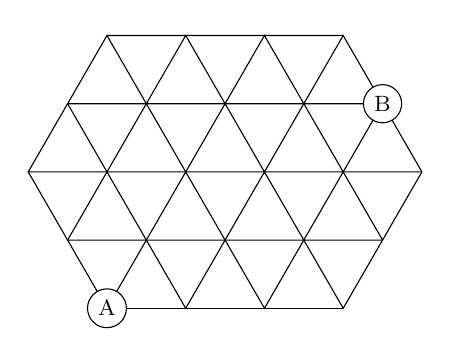
\begin{tikzpicture}\footnotesize
\draw(0,0)--++(1,0)node[sloped,midway]{$\blacktriangleleft$}
          --++(1,0)node[sloped,midway]{$\blacktriangleleft$}
          --++(1,0)node[sloped,midway]{$\blacktriangleleft$};
\draw(0,0)--++(120:1)node[sloped,midway]{$\blacktriangleleft$}
          --++(1,0)node[sloped,midway]{$\blacktriangleright$}
          --++(1,0)node[sloped,midway]{$\blacktriangleleft$}
          --++(1,0)node[sloped,midway]{$\blacktriangleleft$}
          --++(1,0)node[sloped,midway]{$\blacktriangleleft$};
\draw(0,0)++(120:1)--++(120:1)node[sloped,midway]{$\blacktriangleleft$}
          --++(1,0)node[sloped,midway]{$\blacktriangleright$}
          --++(1,0)node[sloped,midway]{$\blacktriangleright$}
          --++(1,0)node[sloped,midway]{$\blacktriangleright$}
          --++(1,0)node[sloped,midway]{$\blacktriangleleft$}
          --++(1,0)node[sloped,midway]{$\blacktriangleleft$};
\draw(0,0)++(120:2)--++(60:1)node[sloped,midway]{$\blacktriangleright$}
          --++(1,0)node[sloped,midway]{$\blacktriangleleft$}
          --++(1,0)node[sloped,midway]{$\blacktriangleleft$}
          --++(1,0)node[sloped,midway]{$\blacktriangleleft$}
          --++(1,0)node[sloped,midway]{$\blacktriangleleft$};
\draw(0,0)++(120:2)++(60:1)--++(60:1)node[sloped,midway]{$\blacktriangleright$}
          --++(1,0)node[sloped,midway]{$\blacktriangleright$}
          --++(1,0)node[sloped,midway]{$\blacktriangleright$}
          --++(1,0)node[sloped,midway]{$\blacktriangleright$};
\draw(0,0)--++(60:1)node[sloped,midway]{$\blacktriangleleft$}
          --++(-60:1)node[sloped,midway]{$\blacktriangleright$}
          --++(60:1)node[sloped,midway]{$\blacktriangleright$}
          --++(-60:1)node[sloped,midway]{$\blacktriangleleft$}
          --++(60:1)node[sloped,midway]{$\blacktriangleright$}
          --++(-60:1)node[sloped,midway]{$\blacktriangleleft$}
          --++(60:1)node[sloped,midway]{$\blacktriangleleft$};
\draw(0,0)++(120:1)--++(60:1)node[sloped,midway]{$\blacktriangleright$}
          --++(-60:1)node[sloped,midway]{$\blacktriangleright$}
          --++(60:1)node[sloped,midway]{$\blacktriangleleft$}
          --++(-60:1)node[sloped,midway]{$\blacktriangleright$}
          --++(60:1)node[sloped,midway]{$\blacktriangleright$}
          --++(-60:1)node[sloped,midway]{$\blacktriangleright$}
          --++(60:1)node[sloped,midway]{$\blacktriangleright$}
          --++(-60:1)node[sloped,midway]{$\blacktriangleleft$}
          --++(60:1)node[sloped,midway]{$\blacktriangleleft$};
\draw(0,0)++(120:2)++(60:1)--++(-60:1)node[sloped,midway]{$\blacktriangleright$}
          --++(60:1)node[sloped,midway]{$\blacktriangleright$}
          --++(-60:1)node[sloped,midway]{$\blacktriangleright$}
          --++(60:1)node[sloped,midway]{$\blacktriangleleft$}
          --++(-60:1)node[sloped,midway]{$\blacktriangleright$}
          --++(60:1)node[sloped,midway]{$\blacktriangleright$}
          --++(-60:1)node[sloped,midway]{$\blacktriangleleft$}
          --++(60:1)node[sloped,midway]{$\blacktriangleright$}
          --++(-60:1)node[sloped,midway]{$\blacktriangleright$};
\draw(0,0)++(120:2)++(60:2)--++(-60:1)node[sloped,midway]{$\blacktriangleright$}
          --++(60:1)node[sloped,midway]{$\blacktriangleright$}
          --++(-60:1)node[sloped,midway]{$\blacktriangleright$}
          --++(60:1)node[sloped,midway]{$\blacktriangleleft$}
          --++(-60:1)node[sloped,midway]{$\blacktriangleleft$}
          --++(60:1)node[sloped,midway]{$\blacktriangleright$}
          --++(-60:1)node[sloped,midway]{$\blacktriangleright$};
\node[circle,draw,inner sep = 2pt,fill=white]at(0,0){A};
\draw(0,0)++(2,0)++(60:3)node[circle,draw,inner sep = 2pt,fill=white]{B};
\end{tikzpicture}\par}

Pour être sûr de trouver le chemin le plus court, il faudrait explorer tous les chemins et retenir le plus court. On peut commencer à la main :

\begin{multicols}{4}
\begin{center}
\begin{tikzpicture}[scale=0.5]\footnotesize
\draw[line width=3pt,color=rouge](0,0)--++(120:2)--++(60:2)--++(3,0)--++(-60:1);
\node[below right]at(0,0){longueur : 8};
\draw(0,0)--++(1,0)node[sloped,midway,scale=0.5]{$\blacktriangleleft$}
          --++(1,0)node[sloped,midway,scale=0.5]{$\blacktriangleleft$}
          --++(1,0)node[sloped,midway,scale=0.5]{$\blacktriangleleft$};
\draw(0,0)--++(120:1)node[sloped,midway,scale=0.5]{$\blacktriangleleft$}
          --++(1,0)node[sloped,midway,scale=0.5]{$\blacktriangleright$}
          --++(1,0)node[sloped,midway,scale=0.5]{$\blacktriangleleft$}
          --++(1,0)node[sloped,midway,scale=0.5]{$\blacktriangleleft$}
          --++(1,0)node[sloped,midway,scale=0.5]{$\blacktriangleleft$};
\draw(0,0)++(120:1)--++(120:1)node[sloped,midway,scale=0.5]{$\blacktriangleleft$}
          --++(1,0)node[sloped,midway,scale=0.5]{$\blacktriangleright$}
          --++(1,0)node[sloped,midway,scale=0.5]{$\blacktriangleright$}
          --++(1,0)node[sloped,midway,scale=0.5]{$\blacktriangleright$}
          --++(1,0)node[sloped,midway,scale=0.5]{$\blacktriangleleft$}
          --++(1,0)node[sloped,midway,scale=0.5]{$\blacktriangleleft$};
\draw(0,0)++(120:2)--++(60:1)node[sloped,midway,scale=0.5]{$\blacktriangleright$}
          --++(1,0)node[sloped,midway,scale=0.5]{$\blacktriangleleft$}
          --++(1,0)node[sloped,midway,scale=0.5]{$\blacktriangleleft$}
          --++(1,0)node[sloped,midway,scale=0.5]{$\blacktriangleleft$}
          --++(1,0)node[sloped,midway,scale=0.5]{$\blacktriangleleft$};
\draw(0,0)++(120:2)++(60:1)--++(60:1)node[sloped,midway,scale=0.5]{$\blacktriangleright$}
          --++(1,0)node[sloped,midway,scale=0.5]{$\blacktriangleright$}
          --++(1,0)node[sloped,midway,scale=0.5]{$\blacktriangleright$}
          --++(1,0)node[sloped,midway,scale=0.5]{$\blacktriangleright$};
\draw(0,0)--++(60:1)node[sloped,midway,scale=0.5]{$\blacktriangleleft$}
          --++(-60:1)node[sloped,midway,scale=0.5]{$\blacktriangleright$}
          --++(60:1)node[sloped,midway,scale=0.5]{$\blacktriangleright$}
          --++(-60:1)node[sloped,midway,scale=0.5]{$\blacktriangleleft$}
          --++(60:1)node[sloped,midway,scale=0.5]{$\blacktriangleright$}
          --++(-60:1)node[sloped,midway,scale=0.5]{$\blacktriangleleft$}
          --++(60:1)node[sloped,midway,scale=0.5]{$\blacktriangleleft$};
\draw(0,0)++(120:1)--++(60:1)node[sloped,midway,scale=0.5]{$\blacktriangleright$}
          --++(-60:1)node[sloped,midway,scale=0.5]{$\blacktriangleright$}
          --++(60:1)node[sloped,midway,scale=0.5]{$\blacktriangleleft$}
          --++(-60:1)node[sloped,midway,scale=0.5]{$\blacktriangleright$}
          --++(60:1)node[sloped,midway,scale=0.5]{$\blacktriangleright$}
          --++(-60:1)node[sloped,midway,scale=0.5]{$\blacktriangleright$}
          --++(60:1)node[sloped,midway,scale=0.5]{$\blacktriangleright$}
          --++(-60:1)node[sloped,midway,scale=0.5]{$\blacktriangleleft$}
          --++(60:1)node[sloped,midway,scale=0.5]{$\blacktriangleleft$};
\draw(0,0)++(120:2)++(60:1)--++(-60:1)node[sloped,midway,scale=0.5]{$\blacktriangleright$}
          --++(60:1)node[sloped,midway,scale=0.5]{$\blacktriangleright$}
          --++(-60:1)node[sloped,midway,scale=0.5]{$\blacktriangleright$}
          --++(60:1)node[sloped,midway,scale=0.5]{$\blacktriangleleft$}
          --++(-60:1)node[sloped,midway,scale=0.5]{$\blacktriangleright$}
          --++(60:1)node[sloped,midway,scale=0.5]{$\blacktriangleright$}
          --++(-60:1)node[sloped,midway,scale=0.5]{$\blacktriangleleft$}
          --++(60:1)node[sloped,midway,scale=0.5]{$\blacktriangleright$}
          --++(-60:1)node[sloped,midway,scale=0.5]{$\blacktriangleright$};
\draw(0,0)++(120:2)++(60:2)--++(-60:1)node[sloped,midway,scale=0.5]{$\blacktriangleright$}
          --++(60:1)node[sloped,midway,scale=0.5]{$\blacktriangleright$}
          --++(-60:1)node[sloped,midway,scale=0.5]{$\blacktriangleright$}
          --++(60:1)node[sloped,midway,scale=0.5]{$\blacktriangleleft$}
          --++(-60:1)node[sloped,midway,scale=0.5]{$\blacktriangleleft$}
          --++(60:1)node[sloped,midway,scale=0.5]{$\blacktriangleright$}
          --++(-60:1)node[sloped,midway,scale=0.5]{$\blacktriangleright$};
\node[circle,draw,inner sep = 1pt,fill=white,scale=0.5]at(0,0){A};
\draw(0,0)++(2,0)++(60:3)node[circle,draw,inner sep = 1pt,fill=white,scale=0.5]{B};
\end{tikzpicture}

\begin{tikzpicture}[scale=0.5]\footnotesize
\draw[line width=3pt,color=rouge](0,0)--++(120:1)--++(60:3)--++(-60:3)--++(60:2);
\node[below right]at(0,0){longueur : 9};
\draw(0,0)--++(1,0)node[sloped,midway,scale=0.5]{$\blacktriangleleft$}
          --++(1,0)node[sloped,midway,scale=0.5]{$\blacktriangleleft$}
          --++(1,0)node[sloped,midway,scale=0.5]{$\blacktriangleleft$};
\draw(0,0)--++(120:1)node[sloped,midway,scale=0.5]{$\blacktriangleleft$}
          --++(1,0)node[sloped,midway,scale=0.5]{$\blacktriangleright$}
          --++(1,0)node[sloped,midway,scale=0.5]{$\blacktriangleleft$}
          --++(1,0)node[sloped,midway,scale=0.5]{$\blacktriangleleft$}
          --++(1,0)node[sloped,midway,scale=0.5]{$\blacktriangleleft$};
\draw(0,0)++(120:1)--++(120:1)node[sloped,midway,scale=0.5]{$\blacktriangleleft$}
          --++(1,0)node[sloped,midway,scale=0.5]{$\blacktriangleright$}
          --++(1,0)node[sloped,midway,scale=0.5]{$\blacktriangleright$}
          --++(1,0)node[sloped,midway,scale=0.5]{$\blacktriangleright$}
          --++(1,0)node[sloped,midway,scale=0.5]{$\blacktriangleleft$}
          --++(1,0)node[sloped,midway,scale=0.5]{$\blacktriangleleft$};
\draw(0,0)++(120:2)--++(60:1)node[sloped,midway,scale=0.5]{$\blacktriangleright$}
          --++(1,0)node[sloped,midway,scale=0.5]{$\blacktriangleleft$}
          --++(1,0)node[sloped,midway,scale=0.5]{$\blacktriangleleft$}
          --++(1,0)node[sloped,midway,scale=0.5]{$\blacktriangleleft$}
          --++(1,0)node[sloped,midway,scale=0.5]{$\blacktriangleleft$};
\draw(0,0)++(120:2)++(60:1)--++(60:1)node[sloped,midway,scale=0.5]{$\blacktriangleright$}
          --++(1,0)node[sloped,midway,scale=0.5]{$\blacktriangleright$}
          --++(1,0)node[sloped,midway,scale=0.5]{$\blacktriangleright$}
          --++(1,0)node[sloped,midway,scale=0.5]{$\blacktriangleright$};
\draw(0,0)--++(60:1)node[sloped,midway,scale=0.5]{$\blacktriangleleft$}
          --++(-60:1)node[sloped,midway,scale=0.5]{$\blacktriangleright$}
          --++(60:1)node[sloped,midway,scale=0.5]{$\blacktriangleright$}
          --++(-60:1)node[sloped,midway,scale=0.5]{$\blacktriangleleft$}
          --++(60:1)node[sloped,midway,scale=0.5]{$\blacktriangleright$}
          --++(-60:1)node[sloped,midway,scale=0.5]{$\blacktriangleleft$}
          --++(60:1)node[sloped,midway,scale=0.5]{$\blacktriangleleft$};
\draw(0,0)++(120:1)--++(60:1)node[sloped,midway,scale=0.5]{$\blacktriangleright$}
          --++(-60:1)node[sloped,midway,scale=0.5]{$\blacktriangleright$}
          --++(60:1)node[sloped,midway,scale=0.5]{$\blacktriangleleft$}
          --++(-60:1)node[sloped,midway,scale=0.5]{$\blacktriangleright$}
          --++(60:1)node[sloped,midway,scale=0.5]{$\blacktriangleright$}
          --++(-60:1)node[sloped,midway,scale=0.5]{$\blacktriangleright$}
          --++(60:1)node[sloped,midway,scale=0.5]{$\blacktriangleright$}
          --++(-60:1)node[sloped,midway,scale=0.5]{$\blacktriangleleft$}
          --++(60:1)node[sloped,midway,scale=0.5]{$\blacktriangleleft$};
\draw(0,0)++(120:2)++(60:1)--++(-60:1)node[sloped,midway,scale=0.5]{$\blacktriangleright$}
          --++(60:1)node[sloped,midway,scale=0.5]{$\blacktriangleright$}
          --++(-60:1)node[sloped,midway,scale=0.5]{$\blacktriangleright$}
          --++(60:1)node[sloped,midway,scale=0.5]{$\blacktriangleleft$}
          --++(-60:1)node[sloped,midway,scale=0.5]{$\blacktriangleright$}
          --++(60:1)node[sloped,midway,scale=0.5]{$\blacktriangleright$}
          --++(-60:1)node[sloped,midway,scale=0.5]{$\blacktriangleleft$}
          --++(60:1)node[sloped,midway,scale=0.5]{$\blacktriangleright$}
          --++(-60:1)node[sloped,midway,scale=0.5]{$\blacktriangleright$};
\draw(0,0)++(120:2)++(60:2)--++(-60:1)node[sloped,midway,scale=0.5]{$\blacktriangleright$}
          --++(60:1)node[sloped,midway,scale=0.5]{$\blacktriangleright$}
          --++(-60:1)node[sloped,midway,scale=0.5]{$\blacktriangleright$}
          --++(60:1)node[sloped,midway,scale=0.5]{$\blacktriangleleft$}
          --++(-60:1)node[sloped,midway,scale=0.5]{$\blacktriangleleft$}
          --++(60:1)node[sloped,midway,scale=0.5]{$\blacktriangleright$}
          --++(-60:1)node[sloped,midway,scale=0.5]{$\blacktriangleright$};
\node[circle,draw,inner sep = 1pt,fill=white,scale=0.5]at(0,0){A};
\draw(0,0)++(2,0)++(60:3)node[circle,draw,inner sep = 1pt,fill=white,scale=0.5]{B};
\end{tikzpicture}

\begin{tikzpicture}[scale=0.5]\footnotesize
\draw[line width=3pt,color=rouge](0,0)--++(120:1)--++(1,0)--++(-60:1)--++(60:2)--++(-60:1)--++(60:2);
\node[below right]at(0,0){longueur : 8};
\draw(0,0)--++(1,0)node[sloped,midway,scale=0.5]{$\blacktriangleleft$}
          --++(1,0)node[sloped,midway,scale=0.5]{$\blacktriangleleft$}
          --++(1,0)node[sloped,midway,scale=0.5]{$\blacktriangleleft$};
\draw(0,0)--++(120:1)node[sloped,midway,scale=0.5]{$\blacktriangleleft$}
          --++(1,0)node[sloped,midway,scale=0.5]{$\blacktriangleright$}
          --++(1,0)node[sloped,midway,scale=0.5]{$\blacktriangleleft$}
          --++(1,0)node[sloped,midway,scale=0.5]{$\blacktriangleleft$}
          --++(1,0)node[sloped,midway,scale=0.5]{$\blacktriangleleft$};
\draw(0,0)++(120:1)--++(120:1)node[sloped,midway,scale=0.5]{$\blacktriangleleft$}
          --++(1,0)node[sloped,midway,scale=0.5]{$\blacktriangleright$}
          --++(1,0)node[sloped,midway,scale=0.5]{$\blacktriangleright$}
          --++(1,0)node[sloped,midway,scale=0.5]{$\blacktriangleright$}
          --++(1,0)node[sloped,midway,scale=0.5]{$\blacktriangleleft$}
          --++(1,0)node[sloped,midway,scale=0.5]{$\blacktriangleleft$};
\draw(0,0)++(120:2)--++(60:1)node[sloped,midway,scale=0.5]{$\blacktriangleright$}
          --++(1,0)node[sloped,midway,scale=0.5]{$\blacktriangleleft$}
          --++(1,0)node[sloped,midway,scale=0.5]{$\blacktriangleleft$}
          --++(1,0)node[sloped,midway,scale=0.5]{$\blacktriangleleft$}
          --++(1,0)node[sloped,midway,scale=0.5]{$\blacktriangleleft$};
\draw(0,0)++(120:2)++(60:1)--++(60:1)node[sloped,midway,scale=0.5]{$\blacktriangleright$}
          --++(1,0)node[sloped,midway,scale=0.5]{$\blacktriangleright$}
          --++(1,0)node[sloped,midway,scale=0.5]{$\blacktriangleright$}
          --++(1,0)node[sloped,midway,scale=0.5]{$\blacktriangleright$};
\draw(0,0)--++(60:1)node[sloped,midway,scale=0.5]{$\blacktriangleleft$}
          --++(-60:1)node[sloped,midway,scale=0.5]{$\blacktriangleright$}
          --++(60:1)node[sloped,midway,scale=0.5]{$\blacktriangleright$}
          --++(-60:1)node[sloped,midway,scale=0.5]{$\blacktriangleleft$}
          --++(60:1)node[sloped,midway,scale=0.5]{$\blacktriangleright$}
          --++(-60:1)node[sloped,midway,scale=0.5]{$\blacktriangleleft$}
          --++(60:1)node[sloped,midway,scale=0.5]{$\blacktriangleleft$};
\draw(0,0)++(120:1)--++(60:1)node[sloped,midway,scale=0.5]{$\blacktriangleright$}
          --++(-60:1)node[sloped,midway,scale=0.5]{$\blacktriangleright$}
          --++(60:1)node[sloped,midway,scale=0.5]{$\blacktriangleleft$}
          --++(-60:1)node[sloped,midway,scale=0.5]{$\blacktriangleright$}
          --++(60:1)node[sloped,midway,scale=0.5]{$\blacktriangleright$}
          --++(-60:1)node[sloped,midway,scale=0.5]{$\blacktriangleright$}
          --++(60:1)node[sloped,midway,scale=0.5]{$\blacktriangleright$}
          --++(-60:1)node[sloped,midway,scale=0.5]{$\blacktriangleleft$}
          --++(60:1)node[sloped,midway,scale=0.5]{$\blacktriangleleft$};
\draw(0,0)++(120:2)++(60:1)--++(-60:1)node[sloped,midway,scale=0.5]{$\blacktriangleright$}
          --++(60:1)node[sloped,midway,scale=0.5]{$\blacktriangleright$}
          --++(-60:1)node[sloped,midway,scale=0.5]{$\blacktriangleright$}
          --++(60:1)node[sloped,midway,scale=0.5]{$\blacktriangleleft$}
          --++(-60:1)node[sloped,midway,scale=0.5]{$\blacktriangleright$}
          --++(60:1)node[sloped,midway,scale=0.5]{$\blacktriangleright$}
          --++(-60:1)node[sloped,midway,scale=0.5]{$\blacktriangleleft$}
          --++(60:1)node[sloped,midway,scale=0.5]{$\blacktriangleright$}
          --++(-60:1)node[sloped,midway,scale=0.5]{$\blacktriangleright$};
\draw(0,0)++(120:2)++(60:2)--++(-60:1)node[sloped,midway,scale=0.5]{$\blacktriangleright$}
          --++(60:1)node[sloped,midway,scale=0.5]{$\blacktriangleright$}
          --++(-60:1)node[sloped,midway,scale=0.5]{$\blacktriangleright$}
          --++(60:1)node[sloped,midway,scale=0.5]{$\blacktriangleleft$}
          --++(-60:1)node[sloped,midway,scale=0.5]{$\blacktriangleleft$}
          --++(60:1)node[sloped,midway,scale=0.5]{$\blacktriangleright$}
          --++(-60:1)node[sloped,midway,scale=0.5]{$\blacktriangleright$};
\node[circle,draw,inner sep = 1pt,fill=white,scale=0.5]at(0,0){A};
\draw(0,0)++(2,0)++(60:3)node[circle,draw,inner sep = 1pt,fill=white,scale=0.5]{B};
\end{tikzpicture}

\begin{tikzpicture}[scale=0.5]\footnotesize
\draw[line width=3pt,color=rouge](0,0)--++(120:2)--++(60:2)--++(-60:3)--++(60:3)--++(-60:1);
\node[below right]at(0,0){longueur : 11};
\draw(0,0)--++(1,0)node[sloped,midway,scale=0.5]{$\blacktriangleleft$}
          --++(1,0)node[sloped,midway,scale=0.5]{$\blacktriangleleft$}
          --++(1,0)node[sloped,midway,scale=0.5]{$\blacktriangleleft$};
\draw(0,0)--++(120:1)node[sloped,midway,scale=0.5]{$\blacktriangleleft$}
          --++(1,0)node[sloped,midway,scale=0.5]{$\blacktriangleright$}
          --++(1,0)node[sloped,midway,scale=0.5]{$\blacktriangleleft$}
          --++(1,0)node[sloped,midway,scale=0.5]{$\blacktriangleleft$}
          --++(1,0)node[sloped,midway,scale=0.5]{$\blacktriangleleft$};
\draw(0,0)++(120:1)--++(120:1)node[sloped,midway,scale=0.5]{$\blacktriangleleft$}
          --++(1,0)node[sloped,midway,scale=0.5]{$\blacktriangleright$}
          --++(1,0)node[sloped,midway,scale=0.5]{$\blacktriangleright$}
          --++(1,0)node[sloped,midway,scale=0.5]{$\blacktriangleright$}
          --++(1,0)node[sloped,midway,scale=0.5]{$\blacktriangleleft$}
          --++(1,0)node[sloped,midway,scale=0.5]{$\blacktriangleleft$};
\draw(0,0)++(120:2)--++(60:1)node[sloped,midway,scale=0.5]{$\blacktriangleright$}
          --++(1,0)node[sloped,midway,scale=0.5]{$\blacktriangleleft$}
          --++(1,0)node[sloped,midway,scale=0.5]{$\blacktriangleleft$}
          --++(1,0)node[sloped,midway,scale=0.5]{$\blacktriangleleft$}
          --++(1,0)node[sloped,midway,scale=0.5]{$\blacktriangleleft$};
\draw(0,0)++(120:2)++(60:1)--++(60:1)node[sloped,midway,scale=0.5]{$\blacktriangleright$}
          --++(1,0)node[sloped,midway,scale=0.5]{$\blacktriangleright$}
          --++(1,0)node[sloped,midway,scale=0.5]{$\blacktriangleright$}
          --++(1,0)node[sloped,midway,scale=0.5]{$\blacktriangleright$};
\draw(0,0)--++(60:1)node[sloped,midway,scale=0.5]{$\blacktriangleleft$}
          --++(-60:1)node[sloped,midway,scale=0.5]{$\blacktriangleright$}
          --++(60:1)node[sloped,midway,scale=0.5]{$\blacktriangleright$}
          --++(-60:1)node[sloped,midway,scale=0.5]{$\blacktriangleleft$}
          --++(60:1)node[sloped,midway,scale=0.5]{$\blacktriangleright$}
          --++(-60:1)node[sloped,midway,scale=0.5]{$\blacktriangleleft$}
          --++(60:1)node[sloped,midway,scale=0.5]{$\blacktriangleleft$};
\draw(0,0)++(120:1)--++(60:1)node[sloped,midway,scale=0.5]{$\blacktriangleright$}
          --++(-60:1)node[sloped,midway,scale=0.5]{$\blacktriangleright$}
          --++(60:1)node[sloped,midway,scale=0.5]{$\blacktriangleleft$}
          --++(-60:1)node[sloped,midway,scale=0.5]{$\blacktriangleright$}
          --++(60:1)node[sloped,midway,scale=0.5]{$\blacktriangleright$}
          --++(-60:1)node[sloped,midway,scale=0.5]{$\blacktriangleright$}
          --++(60:1)node[sloped,midway,scale=0.5]{$\blacktriangleright$}
          --++(-60:1)node[sloped,midway,scale=0.5]{$\blacktriangleleft$}
          --++(60:1)node[sloped,midway,scale=0.5]{$\blacktriangleleft$};
\draw(0,0)++(120:2)++(60:1)--++(-60:1)node[sloped,midway,scale=0.5]{$\blacktriangleright$}
          --++(60:1)node[sloped,midway,scale=0.5]{$\blacktriangleright$}
          --++(-60:1)node[sloped,midway,scale=0.5]{$\blacktriangleright$}
          --++(60:1)node[sloped,midway,scale=0.5]{$\blacktriangleleft$}
          --++(-60:1)node[sloped,midway,scale=0.5]{$\blacktriangleright$}
          --++(60:1)node[sloped,midway,scale=0.5]{$\blacktriangleright$}
          --++(-60:1)node[sloped,midway,scale=0.5]{$\blacktriangleleft$}
          --++(60:1)node[sloped,midway,scale=0.5]{$\blacktriangleright$}
          --++(-60:1)node[sloped,midway,scale=0.5]{$\blacktriangleright$};
\draw(0,0)++(120:2)++(60:2)--++(-60:1)node[sloped,midway,scale=0.5]{$\blacktriangleright$}
          --++(60:1)node[sloped,midway,scale=0.5]{$\blacktriangleright$}
          --++(-60:1)node[sloped,midway,scale=0.5]{$\blacktriangleright$}
          --++(60:1)node[sloped,midway,scale=0.5]{$\blacktriangleleft$}
          --++(-60:1)node[sloped,midway,scale=0.5]{$\blacktriangleleft$}
          --++(60:1)node[sloped,midway,scale=0.5]{$\blacktriangleright$}
          --++(-60:1)node[sloped,midway,scale=0.5]{$\blacktriangleright$};
\node[circle,draw,inner sep = 1pt,fill=white,scale=0.5]at(0,0){A};
\draw(0,0)++(2,0)++(60:3)node[circle,draw,inner sep = 1pt,fill=white,scale=0.5]{B};
\end{tikzpicture}\end{center}
\end{multicols}

Dresser la liste de tous les chemins possibles risque d'être long (même pour un ordinateur dans des cas pas forcément très compliqués), mais, à la main, on perçoit, au bout de quelques essais, comment tracer le chemin le plus court. Par exemple on ne repasse jamais deux fois au même endroit, et on va le plus possible emprunter  un chemin horizontal plutôt que deux obliques...

Mais une machine ne << perçoit >> rien. Si on ne veut pas d'un algorithme qui passerait en revue tous les chemins, voilà une possibilité : choisir à chaque étape, et indépendamment de ce qui précède ou suit, la route qui nous rapproche le plus du but.

\begin{multicols}{4}

\begin{tikzpicture}[scale=0.5]\footnotesize
\draw[line width=4pt,color=rouge](0,0)--++(120:1)node{\color{rouge}{$\bullet$}};
\draw(0,0)--++(1,0)node[sloped,midway,scale=0.5]{$\blacktriangleleft$}
          --++(1,0)node[sloped,midway,scale=0.5]{$\blacktriangleleft$}
          --++(1,0)node[sloped,midway,scale=0.5]{$\blacktriangleleft$};
\draw(0,0)--++(120:1)node[sloped,midway,scale=0.5]{$\blacktriangleleft$}
          --++(1,0)node[sloped,midway,scale=0.5]{$\blacktriangleright$}
          --++(1,0)node[sloped,midway,scale=0.5]{$\blacktriangleleft$}
          --++(1,0)node[sloped,midway,scale=0.5]{$\blacktriangleleft$}
          --++(1,0)node[sloped,midway,scale=0.5]{$\blacktriangleleft$};
\draw(0,0)++(120:1)--++(120:1)node[sloped,midway,scale=0.5]{$\blacktriangleleft$}
          --++(1,0)node[sloped,midway,scale=0.5]{$\blacktriangleright$}
          --++(1,0)node[sloped,midway,scale=0.5]{$\blacktriangleright$}
          --++(1,0)node[sloped,midway,scale=0.5]{$\blacktriangleright$}
          --++(1,0)node[sloped,midway,scale=0.5]{$\blacktriangleleft$}
          --++(1,0)node[sloped,midway,scale=0.5]{$\blacktriangleleft$};
\draw(0,0)++(120:2)--++(60:1)node[sloped,midway,scale=0.5]{$\blacktriangleright$}
          --++(1,0)node[sloped,midway,scale=0.5]{$\blacktriangleleft$}
          --++(1,0)node[sloped,midway,scale=0.5]{$\blacktriangleleft$}
          --++(1,0)node[sloped,midway,scale=0.5]{$\blacktriangleleft$}
          --++(1,0)node[sloped,midway,scale=0.5]{$\blacktriangleleft$};
\draw(0,0)++(120:2)++(60:1)--++(60:1)node[sloped,midway,scale=0.5]{$\blacktriangleright$}
          --++(1,0)node[sloped,midway,scale=0.5]{$\blacktriangleright$}
          --++(1,0)node[sloped,midway,scale=0.5]{$\blacktriangleright$}
          --++(1,0)node[sloped,midway,scale=0.5]{$\blacktriangleright$};
\draw(0,0)--++(60:1)node[sloped,midway,scale=0.5]{$\blacktriangleleft$}
          --++(-60:1)node[sloped,midway,scale=0.5]{$\blacktriangleright$}
          --++(60:1)node[sloped,midway,scale=0.5]{$\blacktriangleright$}
          --++(-60:1)node[sloped,midway,scale=0.5]{$\blacktriangleleft$}
          --++(60:1)node[sloped,midway,scale=0.5]{$\blacktriangleright$}
          --++(-60:1)node[sloped,midway,scale=0.5]{$\blacktriangleleft$}
          --++(60:1)node[sloped,midway,scale=0.5]{$\blacktriangleleft$};
\draw(0,0)++(120:1)--++(60:1)node[sloped,midway,scale=0.5]{$\blacktriangleright$}
          --++(-60:1)node[sloped,midway,scale=0.5]{$\blacktriangleright$}
          --++(60:1)node[sloped,midway,scale=0.5]{$\blacktriangleleft$}
          --++(-60:1)node[sloped,midway,scale=0.5]{$\blacktriangleright$}
          --++(60:1)node[sloped,midway,scale=0.5]{$\blacktriangleright$}
          --++(-60:1)node[sloped,midway,scale=0.5]{$\blacktriangleright$}
          --++(60:1)node[sloped,midway,scale=0.5]{$\blacktriangleright$}
          --++(-60:1)node[sloped,midway,scale=0.5]{$\blacktriangleleft$}
          --++(60:1)node[sloped,midway,scale=0.5]{$\blacktriangleleft$};
\draw(0,0)++(120:2)++(60:1)--++(-60:1)node[sloped,midway,scale=0.5]{$\blacktriangleright$}
          --++(60:1)node[sloped,midway,scale=0.5]{$\blacktriangleright$}
          --++(-60:1)node[sloped,midway,scale=0.5]{$\blacktriangleright$}
          --++(60:1)node[sloped,midway,scale=0.5]{$\blacktriangleleft$}
          --++(-60:1)node[sloped,midway,scale=0.5]{$\blacktriangleright$}
          --++(60:1)node[sloped,midway,scale=0.5]{$\blacktriangleright$}
          --++(-60:1)node[sloped,midway,scale=0.5]{$\blacktriangleleft$}
          --++(60:1)node[sloped,midway,scale=0.5]{$\blacktriangleright$}
          --++(-60:1)node[sloped,midway,scale=0.5]{$\blacktriangleright$};
\draw(0,0)++(120:2)++(60:2)--++(-60:1)node[sloped,midway,scale=0.5]{$\blacktriangleright$}
          --++(60:1)node[sloped,midway,scale=0.5]{$\blacktriangleright$}
          --++(-60:1)node[sloped,midway,scale=0.5]{$\blacktriangleright$}
          --++(60:1)node[sloped,midway,scale=0.5]{$\blacktriangleleft$}
          --++(-60:1)node[sloped,midway,scale=0.5]{$\blacktriangleleft$}
          --++(60:1)node[sloped,midway,scale=0.5]{$\blacktriangleright$}
          --++(-60:1)node[sloped,midway,scale=0.5]{$\blacktriangleright$};
\clip(-1.25,-0.25)rectangle(4.25,3.75);
\fill[rouge,opacity=0.33](0,0)++(2,0)++(60:3)circle({sqrt(12)});
\draw(0,0)++(2,0)++(60:3)circle({sqrt(12)});
\node[circle,draw,inner sep = 1pt,fill=white,scale=0.5]at(0,0){A};
\draw(0,0)++(2,0)++(60:3)node[circle,draw,inner sep = 1pt,fill=white,scale=0.5]{B};
\node[left=0.25cm]at(0,0){1};
\end{tikzpicture}

\begin{tikzpicture}[scale=0.5]\footnotesize
\draw[line width=3pt,color=rouge](0,0)--++(120:1)--++(1,0)node{\color{rouge}{$\bullet$}};
\draw(0,0)--++(1,0)node[sloped,midway,scale=0.5]{$\blacktriangleleft$}
          --++(1,0)node[sloped,midway,scale=0.5]{$\blacktriangleleft$}
          --++(1,0)node[sloped,midway,scale=0.5]{$\blacktriangleleft$};
\draw(0,0)--++(120:1)node[sloped,midway,scale=0.5]{$\blacktriangleleft$}
          --++(1,0)node[sloped,midway,scale=0.5]{$\blacktriangleright$}
          --++(1,0)node[sloped,midway,scale=0.5]{$\blacktriangleleft$}
          --++(1,0)node[sloped,midway,scale=0.5]{$\blacktriangleleft$}
          --++(1,0)node[sloped,midway,scale=0.5]{$\blacktriangleleft$};
\draw(0,0)++(120:1)--++(120:1)node[sloped,midway,scale=0.5]{$\blacktriangleleft$}
          --++(1,0)node[sloped,midway,scale=0.5]{$\blacktriangleright$}
          --++(1,0)node[sloped,midway,scale=0.5]{$\blacktriangleright$}
          --++(1,0)node[sloped,midway,scale=0.5]{$\blacktriangleright$}
          --++(1,0)node[sloped,midway,scale=0.5]{$\blacktriangleleft$}
          --++(1,0)node[sloped,midway,scale=0.5]{$\blacktriangleleft$};
\draw(0,0)++(120:2)--++(60:1)node[sloped,midway,scale=0.5]{$\blacktriangleright$}
          --++(1,0)node[sloped,midway,scale=0.5]{$\blacktriangleleft$}
          --++(1,0)node[sloped,midway,scale=0.5]{$\blacktriangleleft$}
          --++(1,0)node[sloped,midway,scale=0.5]{$\blacktriangleleft$}
          --++(1,0)node[sloped,midway,scale=0.5]{$\blacktriangleleft$};
\draw(0,0)++(120:2)++(60:1)--++(60:1)node[sloped,midway,scale=0.5]{$\blacktriangleright$}
          --++(1,0)node[sloped,midway,scale=0.5]{$\blacktriangleright$}
          --++(1,0)node[sloped,midway,scale=0.5]{$\blacktriangleright$}
          --++(1,0)node[sloped,midway,scale=0.5]{$\blacktriangleright$};
\draw(0,0)--++(60:1)node[sloped,midway,scale=0.5]{$\blacktriangleleft$}
          --++(-60:1)node[sloped,midway,scale=0.5]{$\blacktriangleright$}
          --++(60:1)node[sloped,midway,scale=0.5]{$\blacktriangleright$}
          --++(-60:1)node[sloped,midway,scale=0.5]{$\blacktriangleleft$}
          --++(60:1)node[sloped,midway,scale=0.5]{$\blacktriangleright$}
          --++(-60:1)node[sloped,midway,scale=0.5]{$\blacktriangleleft$}
          --++(60:1)node[sloped,midway,scale=0.5]{$\blacktriangleleft$};
\draw(0,0)++(120:1)--++(60:1)node[sloped,midway,scale=0.5]{$\blacktriangleright$}
          --++(-60:1)node[sloped,midway,scale=0.5]{$\blacktriangleright$}
          --++(60:1)node[sloped,midway,scale=0.5]{$\blacktriangleleft$}
          --++(-60:1)node[sloped,midway,scale=0.5]{$\blacktriangleright$}
          --++(60:1)node[sloped,midway,scale=0.5]{$\blacktriangleright$}
          --++(-60:1)node[sloped,midway,scale=0.5]{$\blacktriangleright$}
          --++(60:1)node[sloped,midway,scale=0.5]{$\blacktriangleright$}
          --++(-60:1)node[sloped,midway,scale=0.5]{$\blacktriangleleft$}
          --++(60:1)node[sloped,midway,scale=0.5]{$\blacktriangleleft$};
\draw(0,0)++(120:2)++(60:1)--++(-60:1)node[sloped,midway,scale=0.5]{$\blacktriangleright$}
          --++(60:1)node[sloped,midway,scale=0.5]{$\blacktriangleright$}
          --++(-60:1)node[sloped,midway,scale=0.5]{$\blacktriangleright$}
          --++(60:1)node[sloped,midway,scale=0.5]{$\blacktriangleleft$}
          --++(-60:1)node[sloped,midway,scale=0.5]{$\blacktriangleright$}
          --++(60:1)node[sloped,midway,scale=0.5]{$\blacktriangleright$}
          --++(-60:1)node[sloped,midway,scale=0.5]{$\blacktriangleleft$}
          --++(60:1)node[sloped,midway,scale=0.5]{$\blacktriangleright$}
          --++(-60:1)node[sloped,midway,scale=0.5]{$\blacktriangleright$};
\draw(0,0)++(120:2)++(60:2)--++(-60:1)node[sloped,midway,scale=0.5]{$\blacktriangleright$}
          --++(60:1)node[sloped,midway,scale=0.5]{$\blacktriangleright$}
          --++(-60:1)node[sloped,midway,scale=0.5]{$\blacktriangleright$}
          --++(60:1)node[sloped,midway,scale=0.5]{$\blacktriangleleft$}
          --++(-60:1)node[sloped,midway,scale=0.5]{$\blacktriangleleft$}
          --++(60:1)node[sloped,midway,scale=0.5]{$\blacktriangleright$}
          --++(-60:1)node[sloped,midway,scale=0.5]{$\blacktriangleright$};
\clip(-1.25,-0.25)rectangle(4.25,3.75);
\fill[rouge,opacity=0.33](0,0)++(2,0)++(60:3)circle({sqrt(2.5*2.5+1.5*1.5*3)});
\draw(0,0)++(2,0)++(60:3)circle({sqrt(2.5*2.5+1.5*1.5*3)});
\node[circle,draw,inner sep = 1pt,fill=white,scale=0.5]at(0,0){A};
\draw(0,0)++(2,0)++(60:3)node[circle,draw,inner sep = 1pt,fill=white,scale=0.5]{B};
\node[left=0.25cm]at(0,0){2};
\end{tikzpicture}

\begin{tikzpicture}[scale=0.5]\footnotesize
\draw[line width=3pt,color=rouge](0,0)--++(120:1)--++(1,0)--++(-60:1)node{\color{rouge}{$\bullet$}};
\draw(0,0)--++(1,0)node[sloped,midway,scale=0.5]{$\blacktriangleleft$}
          --++(1,0)node[sloped,midway,scale=0.5]{$\blacktriangleleft$}
          --++(1,0)node[sloped,midway,scale=0.5]{$\blacktriangleleft$};
\draw(0,0)--++(120:1)node[sloped,midway,scale=0.5]{$\blacktriangleleft$}
          --++(1,0)node[sloped,midway,scale=0.5]{$\blacktriangleright$}
          --++(1,0)node[sloped,midway,scale=0.5]{$\blacktriangleleft$}
          --++(1,0)node[sloped,midway,scale=0.5]{$\blacktriangleleft$}
          --++(1,0)node[sloped,midway,scale=0.5]{$\blacktriangleleft$};
\draw(0,0)++(120:1)--++(120:1)node[sloped,midway,scale=0.5]{$\blacktriangleleft$}
          --++(1,0)node[sloped,midway,scale=0.5]{$\blacktriangleright$}
          --++(1,0)node[sloped,midway,scale=0.5]{$\blacktriangleright$}
          --++(1,0)node[sloped,midway,scale=0.5]{$\blacktriangleright$}
          --++(1,0)node[sloped,midway,scale=0.5]{$\blacktriangleleft$}
          --++(1,0)node[sloped,midway,scale=0.5]{$\blacktriangleleft$};
\draw(0,0)++(120:2)--++(60:1)node[sloped,midway,scale=0.5]{$\blacktriangleright$}
          --++(1,0)node[sloped,midway,scale=0.5]{$\blacktriangleleft$}
          --++(1,0)node[sloped,midway,scale=0.5]{$\blacktriangleleft$}
          --++(1,0)node[sloped,midway,scale=0.5]{$\blacktriangleleft$}
          --++(1,0)node[sloped,midway,scale=0.5]{$\blacktriangleleft$};
\draw(0,0)++(120:2)++(60:1)--++(60:1)node[sloped,midway,scale=0.5]{$\blacktriangleright$}
          --++(1,0)node[sloped,midway,scale=0.5]{$\blacktriangleright$}
          --++(1,0)node[sloped,midway,scale=0.5]{$\blacktriangleright$}
          --++(1,0)node[sloped,midway,scale=0.5]{$\blacktriangleright$};
\draw(0,0)--++(60:1)node[sloped,midway,scale=0.5]{$\blacktriangleleft$}
          --++(-60:1)node[sloped,midway,scale=0.5]{$\blacktriangleright$}
          --++(60:1)node[sloped,midway,scale=0.5]{$\blacktriangleright$}
          --++(-60:1)node[sloped,midway,scale=0.5]{$\blacktriangleleft$}
          --++(60:1)node[sloped,midway,scale=0.5]{$\blacktriangleright$}
          --++(-60:1)node[sloped,midway,scale=0.5]{$\blacktriangleleft$}
          --++(60:1)node[sloped,midway,scale=0.5]{$\blacktriangleleft$};
\draw(0,0)++(120:1)--++(60:1)node[sloped,midway,scale=0.5]{$\blacktriangleright$}
          --++(-60:1)node[sloped,midway,scale=0.5]{$\blacktriangleright$}
          --++(60:1)node[sloped,midway,scale=0.5]{$\blacktriangleleft$}
          --++(-60:1)node[sloped,midway,scale=0.5]{$\blacktriangleright$}
          --++(60:1)node[sloped,midway,scale=0.5]{$\blacktriangleright$}
          --++(-60:1)node[sloped,midway,scale=0.5]{$\blacktriangleright$}
          --++(60:1)node[sloped,midway,scale=0.5]{$\blacktriangleright$}
          --++(-60:1)node[sloped,midway,scale=0.5]{$\blacktriangleleft$}
          --++(60:1)node[sloped,midway,scale=0.5]{$\blacktriangleleft$};
\draw(0,0)++(120:2)++(60:1)--++(-60:1)node[sloped,midway,scale=0.5]{$\blacktriangleright$}
          --++(60:1)node[sloped,midway,scale=0.5]{$\blacktriangleright$}
          --++(-60:1)node[sloped,midway,scale=0.5]{$\blacktriangleright$}
          --++(60:1)node[sloped,midway,scale=0.5]{$\blacktriangleleft$}
          --++(-60:1)node[sloped,midway,scale=0.5]{$\blacktriangleright$}
          --++(60:1)node[sloped,midway,scale=0.5]{$\blacktriangleright$}
          --++(-60:1)node[sloped,midway,scale=0.5]{$\blacktriangleleft$}
          --++(60:1)node[sloped,midway,scale=0.5]{$\blacktriangleright$}
          --++(-60:1)node[sloped,midway,scale=0.5]{$\blacktriangleright$};
\draw(0,0)++(120:2)++(60:2)--++(-60:1)node[sloped,midway,scale=0.5]{$\blacktriangleright$}
          --++(60:1)node[sloped,midway,scale=0.5]{$\blacktriangleright$}
          --++(-60:1)node[sloped,midway,scale=0.5]{$\blacktriangleright$}
          --++(60:1)node[sloped,midway,scale=0.5]{$\blacktriangleleft$}
          --++(-60:1)node[sloped,midway,scale=0.5]{$\blacktriangleleft$}
          --++(60:1)node[sloped,midway,scale=0.5]{$\blacktriangleright$}
          --++(-60:1)node[sloped,midway,scale=0.5]{$\blacktriangleright$};
\clip(-1.25,-0.25)rectangle(4.25,3.75);
\fill[rouge,opacity=0.33](0,0)++(2,0)++(60:3)circle({sqrt(7)});
\draw(0,0)++(2,0)++(60:3)circle({sqrt(7)});
\node[circle,draw,inner sep = 1pt,fill=white,scale=0.5]at(0,0){A};
\draw(0,0)++(2,0)++(60:3)node[circle,draw,inner sep = 1pt,fill=white,scale=0.5]{B};
\node[left=0.25cm]at(0,0){3};
\end{tikzpicture}

\begin{tikzpicture}[scale=0.5]\footnotesize
\draw[line width=3pt,color=rouge](0,0)--++(120:1)--++(1,0)--++(-60:1)--++(60:1)node{\color{rouge}{$\bullet$}};
\draw(0,0)--++(1,0)node[sloped,midway,scale=0.5]{$\blacktriangleleft$}
          --++(1,0)node[sloped,midway,scale=0.5]{$\blacktriangleleft$}
          --++(1,0)node[sloped,midway,scale=0.5]{$\blacktriangleleft$};
\draw(0,0)--++(120:1)node[sloped,midway,scale=0.5]{$\blacktriangleleft$}
          --++(1,0)node[sloped,midway,scale=0.5]{$\blacktriangleright$}
          --++(1,0)node[sloped,midway,scale=0.5]{$\blacktriangleleft$}
          --++(1,0)node[sloped,midway,scale=0.5]{$\blacktriangleleft$}
          --++(1,0)node[sloped,midway,scale=0.5]{$\blacktriangleleft$};
\draw(0,0)++(120:1)--++(120:1)node[sloped,midway,scale=0.5]{$\blacktriangleleft$}
          --++(1,0)node[sloped,midway,scale=0.5]{$\blacktriangleright$}
          --++(1,0)node[sloped,midway,scale=0.5]{$\blacktriangleright$}
          --++(1,0)node[sloped,midway,scale=0.5]{$\blacktriangleright$}
          --++(1,0)node[sloped,midway,scale=0.5]{$\blacktriangleleft$}
          --++(1,0)node[sloped,midway,scale=0.5]{$\blacktriangleleft$};
\draw(0,0)++(120:2)--++(60:1)node[sloped,midway,scale=0.5]{$\blacktriangleright$}
          --++(1,0)node[sloped,midway,scale=0.5]{$\blacktriangleleft$}
          --++(1,0)node[sloped,midway,scale=0.5]{$\blacktriangleleft$}
          --++(1,0)node[sloped,midway,scale=0.5]{$\blacktriangleleft$}
          --++(1,0)node[sloped,midway,scale=0.5]{$\blacktriangleleft$};
\draw(0,0)++(120:2)++(60:1)--++(60:1)node[sloped,midway,scale=0.5]{$\blacktriangleright$}
          --++(1,0)node[sloped,midway,scale=0.5]{$\blacktriangleright$}
          --++(1,0)node[sloped,midway,scale=0.5]{$\blacktriangleright$}
          --++(1,0)node[sloped,midway,scale=0.5]{$\blacktriangleright$};
\draw(0,0)--++(60:1)node[sloped,midway,scale=0.5]{$\blacktriangleleft$}
          --++(-60:1)node[sloped,midway,scale=0.5]{$\blacktriangleright$}
          --++(60:1)node[sloped,midway,scale=0.5]{$\blacktriangleright$}
          --++(-60:1)node[sloped,midway,scale=0.5]{$\blacktriangleleft$}
          --++(60:1)node[sloped,midway,scale=0.5]{$\blacktriangleright$}
          --++(-60:1)node[sloped,midway,scale=0.5]{$\blacktriangleleft$}
          --++(60:1)node[sloped,midway,scale=0.5]{$\blacktriangleleft$};
\draw(0,0)++(120:1)--++(60:1)node[sloped,midway,scale=0.5]{$\blacktriangleright$}
          --++(-60:1)node[sloped,midway,scale=0.5]{$\blacktriangleright$}
          --++(60:1)node[sloped,midway,scale=0.5]{$\blacktriangleleft$}
          --++(-60:1)node[sloped,midway,scale=0.5]{$\blacktriangleright$}
          --++(60:1)node[sloped,midway,scale=0.5]{$\blacktriangleright$}
          --++(-60:1)node[sloped,midway,scale=0.5]{$\blacktriangleright$}
          --++(60:1)node[sloped,midway,scale=0.5]{$\blacktriangleright$}
          --++(-60:1)node[sloped,midway,scale=0.5]{$\blacktriangleleft$}
          --++(60:1)node[sloped,midway,scale=0.5]{$\blacktriangleleft$};
\draw(0,0)++(120:2)++(60:1)--++(-60:1)node[sloped,midway,scale=0.5]{$\blacktriangleright$}
          --++(60:1)node[sloped,midway,scale=0.5]{$\blacktriangleright$}
          --++(-60:1)node[sloped,midway,scale=0.5]{$\blacktriangleright$}
          --++(60:1)node[sloped,midway,scale=0.5]{$\blacktriangleleft$}
          --++(-60:1)node[sloped,midway,scale=0.5]{$\blacktriangleright$}
          --++(60:1)node[sloped,midway,scale=0.5]{$\blacktriangleright$}
          --++(-60:1)node[sloped,midway,scale=0.5]{$\blacktriangleleft$}
          --++(60:1)node[sloped,midway,scale=0.5]{$\blacktriangleright$}
          --++(-60:1)node[sloped,midway,scale=0.5]{$\blacktriangleright$};
\draw(0,0)++(120:2)++(60:2)--++(-60:1)node[sloped,midway,scale=0.5]{$\blacktriangleright$}
          --++(60:1)node[sloped,midway,scale=0.5]{$\blacktriangleright$}
          --++(-60:1)node[sloped,midway,scale=0.5]{$\blacktriangleright$}
          --++(60:1)node[sloped,midway,scale=0.5]{$\blacktriangleleft$}
          --++(-60:1)node[sloped,midway,scale=0.5]{$\blacktriangleleft$}
          --++(60:1)node[sloped,midway,scale=0.5]{$\blacktriangleright$}
          --++(-60:1)node[sloped,midway,scale=0.5]{$\blacktriangleright$};
\clip(-1.25,-0.25)rectangle(4.25,3.75);
\fill[rouge,opacity=0.33](0,0)++(2,0)++(60:3)circle({sqrt(1.5*1.5+3*0.5*0.5)});
\draw(0,0)++(2,0)++(60:3)circle({sqrt(1.5*1.5+3*0.5*0.5)});
\node[circle,draw,inner sep = 1pt,fill=white,scale=0.5]at(0,0){A};
\draw(0,0)++(2,0)++(60:3)node[circle,draw,inner sep = 1pt,fill=white,scale=0.5]{B};
\node[left=0.25cm]at(0,0){4};
\end{tikzpicture}
\end{multicols}

\begin{multicols}{4}
\begin{tikzpicture}[scale=0.5]\footnotesize
\draw[line width=3pt,color=rouge](0,0)--++(120:1)--++(1,0)--++(-60:1)--++(60:2)node{\color{rouge}{$\bullet$}};
\draw(0,0)--++(1,0)node[sloped,midway,scale=0.5]{$\blacktriangleleft$}
          --++(1,0)node[sloped,midway,scale=0.5]{$\blacktriangleleft$}
          --++(1,0)node[sloped,midway,scale=0.5]{$\blacktriangleleft$};
\draw(0,0)--++(120:1)node[sloped,midway,scale=0.5]{$\blacktriangleleft$}
          --++(1,0)node[sloped,midway,scale=0.5]{$\blacktriangleright$}
          --++(1,0)node[sloped,midway,scale=0.5]{$\blacktriangleleft$}
          --++(1,0)node[sloped,midway,scale=0.5]{$\blacktriangleleft$}
          --++(1,0)node[sloped,midway,scale=0.5]{$\blacktriangleleft$};
\draw(0,0)++(120:1)--++(120:1)node[sloped,midway,scale=0.5]{$\blacktriangleleft$}
          --++(1,0)node[sloped,midway,scale=0.5]{$\blacktriangleright$}
          --++(1,0)node[sloped,midway,scale=0.5]{$\blacktriangleright$}
          --++(1,0)node[sloped,midway,scale=0.5]{$\blacktriangleright$}
          --++(1,0)node[sloped,midway,scale=0.5]{$\blacktriangleleft$}
          --++(1,0)node[sloped,midway,scale=0.5]{$\blacktriangleleft$};
\draw(0,0)++(120:2)--++(60:1)node[sloped,midway,scale=0.5]{$\blacktriangleright$}
          --++(1,0)node[sloped,midway,scale=0.5]{$\blacktriangleleft$}
          --++(1,0)node[sloped,midway,scale=0.5]{$\blacktriangleleft$}
          --++(1,0)node[sloped,midway,scale=0.5]{$\blacktriangleleft$}
          --++(1,0)node[sloped,midway,scale=0.5]{$\blacktriangleleft$};
\draw(0,0)++(120:2)++(60:1)--++(60:1)node[sloped,midway,scale=0.5]{$\blacktriangleright$}
          --++(1,0)node[sloped,midway,scale=0.5]{$\blacktriangleright$}
          --++(1,0)node[sloped,midway,scale=0.5]{$\blacktriangleright$}
          --++(1,0)node[sloped,midway,scale=0.5]{$\blacktriangleright$};
\draw(0,0)--++(60:1)node[sloped,midway,scale=0.5]{$\blacktriangleleft$}
          --++(-60:1)node[sloped,midway,scale=0.5]{$\blacktriangleright$}
          --++(60:1)node[sloped,midway,scale=0.5]{$\blacktriangleright$}
          --++(-60:1)node[sloped,midway,scale=0.5]{$\blacktriangleleft$}
          --++(60:1)node[sloped,midway,scale=0.5]{$\blacktriangleright$}
          --++(-60:1)node[sloped,midway,scale=0.5]{$\blacktriangleleft$}
          --++(60:1)node[sloped,midway,scale=0.5]{$\blacktriangleleft$};
\draw(0,0)++(120:1)--++(60:1)node[sloped,midway,scale=0.5]{$\blacktriangleright$}
          --++(-60:1)node[sloped,midway,scale=0.5]{$\blacktriangleright$}
          --++(60:1)node[sloped,midway,scale=0.5]{$\blacktriangleleft$}
          --++(-60:1)node[sloped,midway,scale=0.5]{$\blacktriangleright$}
          --++(60:1)node[sloped,midway,scale=0.5]{$\blacktriangleright$}
          --++(-60:1)node[sloped,midway,scale=0.5]{$\blacktriangleright$}
          --++(60:1)node[sloped,midway,scale=0.5]{$\blacktriangleright$}
          --++(-60:1)node[sloped,midway,scale=0.5]{$\blacktriangleleft$}
          --++(60:1)node[sloped,midway,scale=0.5]{$\blacktriangleleft$};
\draw(0,0)++(120:2)++(60:1)--++(-60:1)node[sloped,midway,scale=0.5]{$\blacktriangleright$}
          --++(60:1)node[sloped,midway,scale=0.5]{$\blacktriangleright$}
          --++(-60:1)node[sloped,midway,scale=0.5]{$\blacktriangleright$}
          --++(60:1)node[sloped,midway,scale=0.5]{$\blacktriangleleft$}
          --++(-60:1)node[sloped,midway,scale=0.5]{$\blacktriangleright$}
          --++(60:1)node[sloped,midway,scale=0.5]{$\blacktriangleright$}
          --++(-60:1)node[sloped,midway,scale=0.5]{$\blacktriangleleft$}
          --++(60:1)node[sloped,midway,scale=0.5]{$\blacktriangleright$}
          --++(-60:1)node[sloped,midway,scale=0.5]{$\blacktriangleright$};
\draw(0,0)++(120:2)++(60:2)--++(-60:1)node[sloped,midway,scale=0.5]{$\blacktriangleright$}
          --++(60:1)node[sloped,midway,scale=0.5]{$\blacktriangleright$}
          --++(-60:1)node[sloped,midway,scale=0.5]{$\blacktriangleright$}
          --++(60:1)node[sloped,midway,scale=0.5]{$\blacktriangleleft$}
          --++(-60:1)node[sloped,midway,scale=0.5]{$\blacktriangleleft$}
          --++(60:1)node[sloped,midway,scale=0.5]{$\blacktriangleright$}
          --++(-60:1)node[sloped,midway,scale=0.5]{$\blacktriangleright$};
\clip(-1.25,-0.25)rectangle(4.25,3.75);
\fill[rouge,opacity=0.33](0,0)++(2,0)++(60:3)circle(1);
\draw(0,0)++(2,0)++(60:3)circle(1);
\node[circle,draw,inner sep = 1pt,fill=white,scale=0.5]at(0,0){A};
\draw(0,0)++(2,0)++(60:3)node[circle,draw,inner sep = 1pt,fill=white,scale=0.5]{B};
\node[left=0.25cm]at(0,0){5};
\end{tikzpicture}

\begin{tikzpicture}[scale=0.5]\footnotesize
\draw[line width=3pt,color=rouge](0,0)--++(120:1)--++(1,0)--++(-60:1)--++(60:3)node{\color{rouge}{$\bullet$}};
\draw(0,0)--++(1,0)node[sloped,midway,scale=0.5]{$\blacktriangleleft$}
          --++(1,0)node[sloped,midway,scale=0.5]{$\blacktriangleleft$}
          --++(1,0)node[sloped,midway,scale=0.5]{$\blacktriangleleft$};
\draw(0,0)--++(120:1)node[sloped,midway,scale=0.5]{$\blacktriangleleft$}
          --++(1,0)node[sloped,midway,scale=0.5]{$\blacktriangleright$}
          --++(1,0)node[sloped,midway,scale=0.5]{$\blacktriangleleft$}
          --++(1,0)node[sloped,midway,scale=0.5]{$\blacktriangleleft$}
          --++(1,0)node[sloped,midway,scale=0.5]{$\blacktriangleleft$};
\draw(0,0)++(120:1)--++(120:1)node[sloped,midway,scale=0.5]{$\blacktriangleleft$}
          --++(1,0)node[sloped,midway,scale=0.5]{$\blacktriangleright$}
          --++(1,0)node[sloped,midway,scale=0.5]{$\blacktriangleright$}
          --++(1,0)node[sloped,midway,scale=0.5]{$\blacktriangleright$}
          --++(1,0)node[sloped,midway,scale=0.5]{$\blacktriangleleft$}
          --++(1,0)node[sloped,midway,scale=0.5]{$\blacktriangleleft$};
\draw(0,0)++(120:2)--++(60:1)node[sloped,midway,scale=0.5]{$\blacktriangleright$}
          --++(1,0)node[sloped,midway,scale=0.5]{$\blacktriangleleft$}
          --++(1,0)node[sloped,midway,scale=0.5]{$\blacktriangleleft$}
          --++(1,0)node[sloped,midway,scale=0.5]{$\blacktriangleleft$}
          --++(1,0)node[sloped,midway,scale=0.5]{$\blacktriangleleft$};
\draw(0,0)++(120:2)++(60:1)--++(60:1)node[sloped,midway,scale=0.5]{$\blacktriangleright$}
          --++(1,0)node[sloped,midway,scale=0.5]{$\blacktriangleright$}
          --++(1,0)node[sloped,midway,scale=0.5]{$\blacktriangleright$}
          --++(1,0)node[sloped,midway,scale=0.5]{$\blacktriangleright$};
\draw(0,0)--++(60:1)node[sloped,midway,scale=0.5]{$\blacktriangleleft$}
          --++(-60:1)node[sloped,midway,scale=0.5]{$\blacktriangleright$}
          --++(60:1)node[sloped,midway,scale=0.5]{$\blacktriangleright$}
          --++(-60:1)node[sloped,midway,scale=0.5]{$\blacktriangleleft$}
          --++(60:1)node[sloped,midway,scale=0.5]{$\blacktriangleright$}
          --++(-60:1)node[sloped,midway,scale=0.5]{$\blacktriangleleft$}
          --++(60:1)node[sloped,midway,scale=0.5]{$\blacktriangleleft$};
\draw(0,0)++(120:1)--++(60:1)node[sloped,midway,scale=0.5]{$\blacktriangleright$}
          --++(-60:1)node[sloped,midway,scale=0.5]{$\blacktriangleright$}
          --++(60:1)node[sloped,midway,scale=0.5]{$\blacktriangleleft$}
          --++(-60:1)node[sloped,midway,scale=0.5]{$\blacktriangleright$}
          --++(60:1)node[sloped,midway,scale=0.5]{$\blacktriangleright$}
          --++(-60:1)node[sloped,midway,scale=0.5]{$\blacktriangleright$}
          --++(60:1)node[sloped,midway,scale=0.5]{$\blacktriangleright$}
          --++(-60:1)node[sloped,midway,scale=0.5]{$\blacktriangleleft$}
          --++(60:1)node[sloped,midway,scale=0.5]{$\blacktriangleleft$};
\draw(0,0)++(120:2)++(60:1)--++(-60:1)node[sloped,midway,scale=0.5]{$\blacktriangleright$}
          --++(60:1)node[sloped,midway,scale=0.5]{$\blacktriangleright$}
          --++(-60:1)node[sloped,midway,scale=0.5]{$\blacktriangleright$}
          --++(60:1)node[sloped,midway,scale=0.5]{$\blacktriangleleft$}
          --++(-60:1)node[sloped,midway,scale=0.5]{$\blacktriangleright$}
          --++(60:1)node[sloped,midway,scale=0.5]{$\blacktriangleright$}
          --++(-60:1)node[sloped,midway,scale=0.5]{$\blacktriangleleft$}
          --++(60:1)node[sloped,midway,scale=0.5]{$\blacktriangleright$}
          --++(-60:1)node[sloped,midway,scale=0.5]{$\blacktriangleright$};
\draw(0,0)++(120:2)++(60:2)--++(-60:1)node[sloped,midway,scale=0.5]{$\blacktriangleright$}
          --++(60:1)node[sloped,midway,scale=0.5]{$\blacktriangleright$}
          --++(-60:1)node[sloped,midway,scale=0.5]{$\blacktriangleright$}
          --++(60:1)node[sloped,midway,scale=0.5]{$\blacktriangleleft$}
          --++(-60:1)node[sloped,midway,scale=0.5]{$\blacktriangleleft$}
          --++(60:1)node[sloped,midway,scale=0.5]{$\blacktriangleright$}
          --++(-60:1)node[sloped,midway,scale=0.5]{$\blacktriangleright$};
\clip(-1.25,-0.25)rectangle(4.25,3.75);
\fill[rouge,opacity=0.33](0,0)++(2,0)++(60:3)circle(1);
\draw(0,0)++(2,0)++(60:3)circle(1);
\node[circle,draw,inner sep = 1pt,fill=white,scale=0.5]at(0,0){A};
\draw(0,0)++(2,0)++(60:3)node[circle,draw,inner sep = 1pt,fill=white,scale=0.5]{B};
\node[left=0.25cm]at(0,0){6};
\end{tikzpicture}

\begin{tikzpicture}[scale=0.5]\footnotesize
\draw[line width=3pt,color=rouge](0,0)--++(120:1)--++(1,0)--++(-60:1)--++(60:4)node{\color{rouge}{$\bullet$}};
\draw(0,0)--++(1,0)node[sloped,midway,scale=0.5]{$\blacktriangleleft$}
          --++(1,0)node[sloped,midway,scale=0.5]{$\blacktriangleleft$}
          --++(1,0)node[sloped,midway,scale=0.5]{$\blacktriangleleft$};
\draw(0,0)--++(120:1)node[sloped,midway,scale=0.5]{$\blacktriangleleft$}
          --++(1,0)node[sloped,midway,scale=0.5]{$\blacktriangleright$}
          --++(1,0)node[sloped,midway,scale=0.5]{$\blacktriangleleft$}
          --++(1,0)node[sloped,midway,scale=0.5]{$\blacktriangleleft$}
          --++(1,0)node[sloped,midway,scale=0.5]{$\blacktriangleleft$};
\draw(0,0)++(120:1)--++(120:1)node[sloped,midway,scale=0.5]{$\blacktriangleleft$}
          --++(1,0)node[sloped,midway,scale=0.5]{$\blacktriangleright$}
          --++(1,0)node[sloped,midway,scale=0.5]{$\blacktriangleright$}
          --++(1,0)node[sloped,midway,scale=0.5]{$\blacktriangleright$}
          --++(1,0)node[sloped,midway,scale=0.5]{$\blacktriangleleft$}
          --++(1,0)node[sloped,midway,scale=0.5]{$\blacktriangleleft$};
\draw(0,0)++(120:2)--++(60:1)node[sloped,midway,scale=0.5]{$\blacktriangleright$}
          --++(1,0)node[sloped,midway,scale=0.5]{$\blacktriangleleft$}
          --++(1,0)node[sloped,midway,scale=0.5]{$\blacktriangleleft$}
          --++(1,0)node[sloped,midway,scale=0.5]{$\blacktriangleleft$}
          --++(1,0)node[sloped,midway,scale=0.5]{$\blacktriangleleft$};
\draw(0,0)++(120:2)++(60:1)--++(60:1)node[sloped,midway,scale=0.5]{$\blacktriangleright$}
          --++(1,0)node[sloped,midway,scale=0.5]{$\blacktriangleright$}
          --++(1,0)node[sloped,midway,scale=0.5]{$\blacktriangleright$}
          --++(1,0)node[sloped,midway,scale=0.5]{$\blacktriangleright$};
\draw(0,0)--++(60:1)node[sloped,midway,scale=0.5]{$\blacktriangleleft$}
          --++(-60:1)node[sloped,midway,scale=0.5]{$\blacktriangleright$}
          --++(60:1)node[sloped,midway,scale=0.5]{$\blacktriangleright$}
          --++(-60:1)node[sloped,midway,scale=0.5]{$\blacktriangleleft$}
          --++(60:1)node[sloped,midway,scale=0.5]{$\blacktriangleright$}
          --++(-60:1)node[sloped,midway,scale=0.5]{$\blacktriangleleft$}
          --++(60:1)node[sloped,midway,scale=0.5]{$\blacktriangleleft$};
\draw(0,0)++(120:1)--++(60:1)node[sloped,midway,scale=0.5]{$\blacktriangleright$}
          --++(-60:1)node[sloped,midway,scale=0.5]{$\blacktriangleright$}
          --++(60:1)node[sloped,midway,scale=0.5]{$\blacktriangleleft$}
          --++(-60:1)node[sloped,midway,scale=0.5]{$\blacktriangleright$}
          --++(60:1)node[sloped,midway,scale=0.5]{$\blacktriangleright$}
          --++(-60:1)node[sloped,midway,scale=0.5]{$\blacktriangleright$}
          --++(60:1)node[sloped,midway,scale=0.5]{$\blacktriangleright$}
          --++(-60:1)node[sloped,midway,scale=0.5]{$\blacktriangleleft$}
          --++(60:1)node[sloped,midway,scale=0.5]{$\blacktriangleleft$};
\draw(0,0)++(120:2)++(60:1)--++(-60:1)node[sloped,midway,scale=0.5]{$\blacktriangleright$}
          --++(60:1)node[sloped,midway,scale=0.5]{$\blacktriangleright$}
          --++(-60:1)node[sloped,midway,scale=0.5]{$\blacktriangleright$}
          --++(60:1)node[sloped,midway,scale=0.5]{$\blacktriangleleft$}
          --++(-60:1)node[sloped,midway,scale=0.5]{$\blacktriangleright$}
          --++(60:1)node[sloped,midway,scale=0.5]{$\blacktriangleright$}
          --++(-60:1)node[sloped,midway,scale=0.5]{$\blacktriangleleft$}
          --++(60:1)node[sloped,midway,scale=0.5]{$\blacktriangleright$}
          --++(-60:1)node[sloped,midway,scale=0.5]{$\blacktriangleright$};
\draw(0,0)++(120:2)++(60:2)--++(-60:1)node[sloped,midway,scale=0.5]{$\blacktriangleright$}
          --++(60:1)node[sloped,midway,scale=0.5]{$\blacktriangleright$}
          --++(-60:1)node[sloped,midway,scale=0.5]{$\blacktriangleright$}
          --++(60:1)node[sloped,midway,scale=0.5]{$\blacktriangleleft$}
          --++(-60:1)node[sloped,midway,scale=0.5]{$\blacktriangleleft$}
          --++(60:1)node[sloped,midway,scale=0.5]{$\blacktriangleright$}
          --++(-60:1)node[sloped,midway,scale=0.5]{$\blacktriangleright$};
\clip(-1.25,-0.25)rectangle(4.25,3.75);
\node[circle,draw,inner sep = 1pt,fill=white,scale=0.5]at(0,0){A};
\draw(0,0)++(2,0)++(60:3)node[circle,draw,inner sep = 1pt,fill=white,scale=0.5]{B};
\node[left=0.25cm]at(0,0){7};
\end{tikzpicture}


\begin{tikzpicture}[scale=0.5]\footnotesize
\draw[line width=3pt,color=rouge](0,0)--++(120:1)--++(1,0)--++(-60:1)--++(60:4)--++(-60:1);
\draw(0,0)--++(1,0)node[sloped,midway,scale=0.5]{$\blacktriangleleft$}
          --++(1,0)node[sloped,midway,scale=0.5]{$\blacktriangleleft$}
          --++(1,0)node[sloped,midway,scale=0.5]{$\blacktriangleleft$};
\draw(0,0)--++(120:1)node[sloped,midway,scale=0.5]{$\blacktriangleleft$}
          --++(1,0)node[sloped,midway,scale=0.5]{$\blacktriangleright$}
          --++(1,0)node[sloped,midway,scale=0.5]{$\blacktriangleleft$}
          --++(1,0)node[sloped,midway,scale=0.5]{$\blacktriangleleft$}
          --++(1,0)node[sloped,midway,scale=0.5]{$\blacktriangleleft$};
\draw(0,0)++(120:1)--++(120:1)node[sloped,midway,scale=0.5]{$\blacktriangleleft$}
          --++(1,0)node[sloped,midway,scale=0.5]{$\blacktriangleright$}
          --++(1,0)node[sloped,midway,scale=0.5]{$\blacktriangleright$}
          --++(1,0)node[sloped,midway,scale=0.5]{$\blacktriangleright$}
          --++(1,0)node[sloped,midway,scale=0.5]{$\blacktriangleleft$}
          --++(1,0)node[sloped,midway,scale=0.5]{$\blacktriangleleft$};
\draw(0,0)++(120:2)--++(60:1)node[sloped,midway,scale=0.5]{$\blacktriangleright$}
          --++(1,0)node[sloped,midway,scale=0.5]{$\blacktriangleleft$}
          --++(1,0)node[sloped,midway,scale=0.5]{$\blacktriangleleft$}
          --++(1,0)node[sloped,midway,scale=0.5]{$\blacktriangleleft$}
          --++(1,0)node[sloped,midway,scale=0.5]{$\blacktriangleleft$};
\draw(0,0)++(120:2)++(60:1)--++(60:1)node[sloped,midway,scale=0.5]{$\blacktriangleright$}
          --++(1,0)node[sloped,midway,scale=0.5]{$\blacktriangleright$}
          --++(1,0)node[sloped,midway,scale=0.5]{$\blacktriangleright$}
          --++(1,0)node[sloped,midway,scale=0.5]{$\blacktriangleright$};
\draw(0,0)--++(60:1)node[sloped,midway,scale=0.5]{$\blacktriangleleft$}
          --++(-60:1)node[sloped,midway,scale=0.5]{$\blacktriangleright$}
          --++(60:1)node[sloped,midway,scale=0.5]{$\blacktriangleright$}
          --++(-60:1)node[sloped,midway,scale=0.5]{$\blacktriangleleft$}
          --++(60:1)node[sloped,midway,scale=0.5]{$\blacktriangleright$}
          --++(-60:1)node[sloped,midway,scale=0.5]{$\blacktriangleleft$}
          --++(60:1)node[sloped,midway,scale=0.5]{$\blacktriangleleft$};
\draw(0,0)++(120:1)--++(60:1)node[sloped,midway,scale=0.5]{$\blacktriangleright$}
          --++(-60:1)node[sloped,midway,scale=0.5]{$\blacktriangleright$}
          --++(60:1)node[sloped,midway,scale=0.5]{$\blacktriangleleft$}
          --++(-60:1)node[sloped,midway,scale=0.5]{$\blacktriangleright$}
          --++(60:1)node[sloped,midway,scale=0.5]{$\blacktriangleright$}
          --++(-60:1)node[sloped,midway,scale=0.5]{$\blacktriangleright$}
          --++(60:1)node[sloped,midway,scale=0.5]{$\blacktriangleright$}
          --++(-60:1)node[sloped,midway,scale=0.5]{$\blacktriangleleft$}
          --++(60:1)node[sloped,midway,scale=0.5]{$\blacktriangleleft$};
\draw(0,0)++(120:2)++(60:1)--++(-60:1)node[sloped,midway,scale=0.5]{$\blacktriangleright$}
          --++(60:1)node[sloped,midway,scale=0.5]{$\blacktriangleright$}
          --++(-60:1)node[sloped,midway,scale=0.5]{$\blacktriangleright$}
          --++(60:1)node[sloped,midway,scale=0.5]{$\blacktriangleleft$}
          --++(-60:1)node[sloped,midway,scale=0.5]{$\blacktriangleright$}
          --++(60:1)node[sloped,midway,scale=0.5]{$\blacktriangleright$}
          --++(-60:1)node[sloped,midway,scale=0.5]{$\blacktriangleleft$}
          --++(60:1)node[sloped,midway,scale=0.5]{$\blacktriangleright$}
          --++(-60:1)node[sloped,midway,scale=0.5]{$\blacktriangleright$};
\draw(0,0)++(120:2)++(60:2)--++(-60:1)node[sloped,midway,scale=0.5]{$\blacktriangleright$}
          --++(60:1)node[sloped,midway,scale=0.5]{$\blacktriangleright$}
          --++(-60:1)node[sloped,midway,scale=0.5]{$\blacktriangleright$}
          --++(60:1)node[sloped,midway,scale=0.5]{$\blacktriangleleft$}
          --++(-60:1)node[sloped,midway,scale=0.5]{$\blacktriangleleft$}
          --++(60:1)node[sloped,midway,scale=0.5]{$\blacktriangleright$}
          --++(-60:1)node[sloped,midway,scale=0.5]{$\blacktriangleright$};
\clip(-1.25,-0.25)rectangle(4.25,3.75);
\node[circle,draw,inner sep = 1pt,fill=white,scale=0.5]at(0,0){A};
\draw(0,0)++(2,0)++(60:3)node[circle,draw,inner sep = 1pt,fill=white,scale=0.5]{B};
\node[left=0.25cm]at(0,0){8};
\end{tikzpicture}
\end{multicols}

Il n'est pas sûr qu'un tel algorithme apporte une solution (il peut se trouver bloqué dans un cul de sac) ni qu'une solution apportée soit optimale, mais on peut garantir les deux, sous certaines conditions. Comme il a, par ailleurs, une bien meilleure complexité que l'énumération totale des possibilités, il est à privilégier dans les cas favorables.

Ici, ce n'était pas le cas : \begin{tikzpicture}[scale=0.5, baseline= (O.base)]\footnotesize
\coordinate(O)at(0,1.5);
\draw[line width=3pt,color=rouge](0,0)--++(120:1)--++(60:1)--++(2,0)--++(-60:1)--++(60:2);
\node[below right]at(0,0){longueur : 7};
\draw(0,0)--++(1,0)node[sloped,midway,scale=0.5]{$\blacktriangleleft$}
          --++(1,0)node[sloped,midway,scale=0.5]{$\blacktriangleleft$}
          --++(1,0)node[sloped,midway,scale=0.5]{$\blacktriangleleft$};
\draw(0,0)--++(120:1)node[sloped,midway,scale=0.5]{$\blacktriangleleft$}
          --++(1,0)node[sloped,midway,scale=0.5]{$\blacktriangleright$}
          --++(1,0)node[sloped,midway,scale=0.5]{$\blacktriangleleft$}
          --++(1,0)node[sloped,midway,scale=0.5]{$\blacktriangleleft$}
          --++(1,0)node[sloped,midway,scale=0.5]{$\blacktriangleleft$};
\draw(0,0)++(120:1)--++(120:1)node[sloped,midway,scale=0.5]{$\blacktriangleleft$}
          --++(1,0)node[sloped,midway,scale=0.5]{$\blacktriangleright$}
          --++(1,0)node[sloped,midway,scale=0.5]{$\blacktriangleright$}
          --++(1,0)node[sloped,midway,scale=0.5]{$\blacktriangleright$}
          --++(1,0)node[sloped,midway,scale=0.5]{$\blacktriangleleft$}
          --++(1,0)node[sloped,midway,scale=0.5]{$\blacktriangleleft$};
\draw(0,0)++(120:2)--++(60:1)node[sloped,midway,scale=0.5]{$\blacktriangleright$}
          --++(1,0)node[sloped,midway,scale=0.5]{$\blacktriangleleft$}
          --++(1,0)node[sloped,midway,scale=0.5]{$\blacktriangleleft$}
          --++(1,0)node[sloped,midway,scale=0.5]{$\blacktriangleleft$}
          --++(1,0)node[sloped,midway,scale=0.5]{$\blacktriangleleft$};
\draw(0,0)++(120:2)++(60:1)--++(60:1)node[sloped,midway,scale=0.5]{$\blacktriangleright$}
          --++(1,0)node[sloped,midway,scale=0.5]{$\blacktriangleright$}
          --++(1,0)node[sloped,midway,scale=0.5]{$\blacktriangleright$}
          --++(1,0)node[sloped,midway,scale=0.5]{$\blacktriangleright$};
\draw(0,0)--++(60:1)node[sloped,midway,scale=0.5]{$\blacktriangleleft$}
          --++(-60:1)node[sloped,midway,scale=0.5]{$\blacktriangleright$}
          --++(60:1)node[sloped,midway,scale=0.5]{$\blacktriangleright$}
          --++(-60:1)node[sloped,midway,scale=0.5]{$\blacktriangleleft$}
          --++(60:1)node[sloped,midway,scale=0.5]{$\blacktriangleright$}
          --++(-60:1)node[sloped,midway,scale=0.5]{$\blacktriangleleft$}
          --++(60:1)node[sloped,midway,scale=0.5]{$\blacktriangleleft$};
\draw(0,0)++(120:1)--++(60:1)node[sloped,midway,scale=0.5]{$\blacktriangleright$}
          --++(-60:1)node[sloped,midway,scale=0.5]{$\blacktriangleright$}
          --++(60:1)node[sloped,midway,scale=0.5]{$\blacktriangleleft$}
          --++(-60:1)node[sloped,midway,scale=0.5]{$\blacktriangleright$}
          --++(60:1)node[sloped,midway,scale=0.5]{$\blacktriangleright$}
          --++(-60:1)node[sloped,midway,scale=0.5]{$\blacktriangleright$}
          --++(60:1)node[sloped,midway,scale=0.5]{$\blacktriangleright$}
          --++(-60:1)node[sloped,midway,scale=0.5]{$\blacktriangleleft$}
          --++(60:1)node[sloped,midway,scale=0.5]{$\blacktriangleleft$};
\draw(0,0)++(120:2)++(60:1)--++(-60:1)node[sloped,midway,scale=0.5]{$\blacktriangleright$}
          --++(60:1)node[sloped,midway,scale=0.5]{$\blacktriangleright$}
          --++(-60:1)node[sloped,midway,scale=0.5]{$\blacktriangleright$}
          --++(60:1)node[sloped,midway,scale=0.5]{$\blacktriangleleft$}
          --++(-60:1)node[sloped,midway,scale=0.5]{$\blacktriangleright$}
          --++(60:1)node[sloped,midway,scale=0.5]{$\blacktriangleright$}
          --++(-60:1)node[sloped,midway,scale=0.5]{$\blacktriangleleft$}
          --++(60:1)node[sloped,midway,scale=0.5]{$\blacktriangleright$}
          --++(-60:1)node[sloped,midway,scale=0.5]{$\blacktriangleright$};
\draw(0,0)++(120:2)++(60:2)--++(-60:1)node[sloped,midway,scale=0.5]{$\blacktriangleright$}
          --++(60:1)node[sloped,midway,scale=0.5]{$\blacktriangleright$}
          --++(-60:1)node[sloped,midway,scale=0.5]{$\blacktriangleright$}
          --++(60:1)node[sloped,midway,scale=0.5]{$\blacktriangleleft$}
          --++(-60:1)node[sloped,midway,scale=0.5]{$\blacktriangleleft$}
          --++(60:1)node[sloped,midway,scale=0.5]{$\blacktriangleright$}
          --++(-60:1)node[sloped,midway,scale=0.5]{$\blacktriangleright$};
\node[circle,draw,inner sep = 1pt,fill=white,scale=0.5]at(0,0){A};
\draw(0,0)++(2,0)++(60:3)node[circle,draw,inner sep = 1pt,fill=white,scale=0.5]{B};
\end{tikzpicture}

\Cours{{\bfseries Algorithme glouton}

Un algorithme est dit \emph{glouton} si

\begin{itemize}
	\item il résout un problème pas à pas,
	\item en faisant à chaque pas le choix du meilleur gain (ou du moindre coût).
\end{itemize}
}

Il tente donc de résoudre des problèmes d'\emph{optimisation}.

Dans la spécification, le rôle sera de trouver le plus ou le moins ... et la postcondition concernera le maximum ou le minimum ...



\section{Problème du rendu de monnaie}

{\bfseries Énoncé :} Comment rendre la monnaie sur une somme $S$ payée avec un montant $M$ en utilisant le moins de pièces possibles.

\medskip

{\bfseries Décontextualisation :} Comment écrire une somme égale à un certain entier $N$ avec un minimum de termes pris, avec répétition, parmi un ensemble fini $P=\{p_1,\ldots,p_k\}$

\medskip
{\bfseries Spécification :} 

\begin{itemize}
	\item {\bfseries Entrée :} Un entier $N$ (à rendre), des entiers dans $P=\{p_1,\ldots,p_k\}$ (pièces).
	\item {\bfseries Sortie :} Des entiers $\{m_1,\ldots,m_k\}$ (multiplicité de chaque pièce).
	\item {\bfseries Rôle :} Écrire $N$ comme la somme d'un minimum de $P=\{p_1,\ldots,p_k\}$.
	\item {\bfseries Précondition :} Tous les entiers en entrée sont strictement positifs.
	\item {\bfseries Postcondition :} $m_1 p_1 + \ldots + m_k p_k =N$ et $m_1 + ... + m_k$ est minimal pour cette égalité.
\end{itemize}

\medskip
{\bfseries Algorithme :} Il consiste à utiliser les plus grosses pièces en premier.


\begin{algorithm}[H]
\Fct{rendre($N$, $P$)}{
  $trier(P)$ \# par ordre décroissant\;
  $M \leftarrow [0,\ldots,0]$\;
  $somme \leftarrow 0$\;
  $i \leftarrow 0$\;
  \Tq{$somme<N$ {\normalfont et} $i<k$}
  {\eSi{$somme + P[i] \leqslant N$}
   { $M[i] \leftarrow M[i] + 1$\;
     $somme \leftarrow somme + P[i]$\;
   }{ $i \leftarrow i + 1$\;
   }
  }
  \Retour{$M$}
}
\end{algorithm}

{\bfseries Correction :} on peut démontrer qu'il termine toujours (Variant : $N-somme + k-i$).

\begin{itemize}
	\item Il est optimal pour le système européen : $P = [5, 2, 1]$. 
	
	(Par exemple $N=8$, donne bien $M=[1,1,1]$.)
	\item Il peut donner une solution non optimale : 
	
	pour $P = [6, 4, 1]$ et $N=8$, on obtient $M=[1,0,2]$ au lieu de $M=[0,2,0]$.
	\item Il peut ne pas donner de solution correcte : 
	
	pour $P = [5, 2]$ et $N=8$, on obtient $M=[1,1]$ au lieu de $M=[0,4]$.
\end{itemize}


{\bfseries Complexité :} 

Dans le pire cas, toutes les pièces sont plus grandes que $N$ sauf la dernière qui vaut $1$. La boucle fait alors ses $N+k$ itérations qui contiennent une dizaine d'opérations.

Donc : $O(N+k)+Tri(k)$

\section{Problème du sac à dos}

{\bfseries Énoncé :} (version « Lupin ») Comment remplir un sac, à capacité limitée, avec les
objets les plus précieux de tailles variés.

\medskip

{\bfseries Décontextualisation :} Quel sous-ensemble de couples (objets) parmi $O=\{o_1,
\ldots,o_k\}$, où $o_i=(v_i, e_i)$ (valeur et encombrement), maximise la somme des $v_i$ tout en ayant une somme de $e_i$ inférieure à $C$ (capacité).

\medskip
{\bfseries Spécification :} 

\begin{itemize}
	\item {\bfseries Entrée :} Ensemble $O$ de couples de nombres positifs et un nombre C.
	\item {\bfseries Sortie :} Sous-ensemble $O'$ de $O$.
	\item {\bfseries Rôle :} Trouver un sous-ensemble $O'$ de $O$ de couples $o_i=(v_i, e_i)$ tel que la somme des $v_i$ soit maximale et celle des $e_i$ inférieure à $C$.
	\item {\bfseries Précondition :} Tous les entiers en entrée sont strictement positifs.
	\item {\bfseries Postcondition :} $O'$ est un sous-ensemble de $O$.
	
	La somme par rapport à la seconde composante des couples de $O'$ est inférieure à $C$.
	
	Si $O''$ est un autre tel sous-ensemble de $O$, la somme par rapport à la première composante des couples de $O''$ est inférieure à celle de $O'$.
\end{itemize}

\medskip
{\bfseries Algorithme :} 

\begin{itemize}
	\item Essayer d'énumérer toutes les possibilités revient pour chacun des $k$ objets à choisir si oui ou non, il faut le prendre. Il y a donc $2^k$ choix possibles. Ce qui donne à cet algorithme une complexité exponentielle !
	\item l'approche gloutonne est tentante, mais comment faire son choix ?
	
	\begin{itemize}
		\item Le plus cher en premier ?
		\item Le moins encombrant en premier ?
		\item \ldots
	\end{itemize}
	
	En fait ce problème est dit << NP-difficile >> et toute approche gloutonne est vouée à l'échec ! 
\end{itemize}



\chapter{Concepts et méthodes}

\section{Complexité}

\Cours{{\bfseries Complexité}

La complexité d'un algorithme est une mesure de sa \emph{consommation de ressources}. Ces ressources peuvent être l'\emph{énergie}, le \emph{temps}, ou encore l'\emph{espace} nécessaire pour arriver au résultat.}

Si l'espace (par exemple pour de l'informatique embarqué) ou l'énergie (lire l'article << Numérique : le grand gâchis énergétique >> \href{https://lejournal.cnrs.fr/articles/numerique-le-grand-gachis-energetique}{https://lejournal.cnrs.fr/articles/numerique-le-grand-gachis-energetique}) sont aussi des mesures fondamentales, nous nous intéresserons ici plus particulièrement au temps.

\medskip

Pour mesurer ce temps, on pourrait s'armer d'un chronomètre et mesurer le temps d'exécution du programme, mais selon la machine, le langage et son compilateur, le système d'exploitation (etc) utilisé, la mesure pourrait beaucoup fluctuer. On va donc mesurer théoriquement ce temps sur les algorithmes.

\subsection{Principe}

\begin{itemize}
	\item On identifie et on note $n$ la taille des données à traiter.
	\item On choisit les opérations significatives.
	\item On compte le nombre de ces opérations en fonction de $n$.
\end{itemize}

On appellera \emph{complexité}, ou \emph{coût}, le nombre obtenu.

\medskip

Quand on travaille avec des données théoriques, on ne peut pas toujours déterminer exactement le nombre d'opérations (à cause des instructions conditionnelles). On peut alors se placer :

\begin{itemize}
	\item dans le meilleur cas (biaisé par des traitements à part de ces cas),
	\item dans un cas moyen (très difficile à déterminer),
	\item dans le pire cas (celui provoquant le plus d'opérations).
\end{itemize}

En première analyse on traitera toujours le pire cas (après l'avoir identifié). 

\subsection{Classe / coût}



Soit un algorithme de complexité $c(n)$ ; et $f(n)$ une autre expression algébrique en $n$.

\begin{center}On dit que $c(n)$ est un << grand $O$ de $f(n)$ >> noté $c(n)=O(f(n))$

s'il existe un coefficient $k$ tel que $c(n)<k\times f(n)$ pour $n$ assez grand.\end{center}

De manière générale, un algorithme de complexité polynômiale est toujours un $O(n^k)$.

\Cours{{\bfseries Classe / coût}

On appelle classe, l'écriture de la complexité sous la forme $O(f(n))$, pour certaines expressions simples de $f(n)$.

$\star$ Coût constant : $O(1)$ \qquad
$\star$ Coût linéaire : $O(n)$ \qquad
$\star$  Coût quadratique : $O(n^2)$
}


Comme un coût constant est dominé par un coût linéaire, lui-même dominé par un coût quadratique, on note les inclusions suivantes des classes : \[O(1) \subset O(n) \subset O(n^2)\]


Une << bonne >> estimation de complexité doit donc donner la plus petite classe.

\medskip

{\bfseries Exemple :} $4n^2+3n+4 = O(n^2)$



\begin{multicols}{2}\centering\def \Xmin {0} \def \Ymin {0} \def \Xmax {10} \def \Ymax {500}
\begin{tikzpicture}[line cap=round, line join=round, >=latex, x=1cm, y=0.02cm, scale=0.5]

\begin{scope}
\clip(\Xmin,\Ymin) rectangle (\Xmax,\Ymax);
	\fill[samples=100,domain=\Xmin:\Xmax,black!5] plot(\x,{30*\x})|-(0,0);
\end{scope}
% Grille
\fill[black!20](\Xmin,0.75) rectangle (\Xmax,1.25);
\draw [color=black, dotted, xstep=1cm, ystep=1cm] (\Xmin,\Ymin) grid (\Xmax,\Ymax);
\draw[->,color=black] (\Xmin,0) -- (\Xmax,0)node[above left]{\footnotesize $n$};
\draw[->,color=black] (0,\Ymin) -- (0.,\Ymax);
\foreach \x in {0,...,\Xmax}
	\draw[shift={(\x,0)},color=black] (0pt,2pt) -- (0pt,-2pt) node[below] {\footnotesize $\x$};
\foreach \y in {0,100,...,\Ymax}
	\draw[shift={(0,\y)},color=black] (2pt,0pt) -- (-2pt,0pt) node[left] {\footnotesize $\y$};
	\foreach \x in {0,...,\Xmax} \node at({\x},{4*\x*\x+3*\x+4}){$\times$};
\foreach \k in {1,5,10,...,30}\node[right]at(10,{\k*10}){$\k n$};
\clip(\Xmin,\Ymin) rectangle (\Xmax,\Ymax);
	\draw[smooth,samples=100,domain=\Xmin:\Xmax,opacity=0.3] plot(\x,{\x});
	\draw[smooth,samples=100,domain=\Xmin:\Xmax,opacity=0.3] plot(\x,{5*\x});
	\draw[smooth,samples=100,domain=\Xmin:\Xmax,opacity=0.3] plot(\x,{10*\x});
	\draw[smooth,samples=100,domain=\Xmin:\Xmax,opacity=0.3] plot(\x,{15*\x});
	\draw[smooth,samples=100,domain=\Xmin:\Xmax,opacity=0.3] plot(\x,{20*\x});
	\draw[smooth,samples=100,domain=\Xmin:\Xmax,opacity=0.3] plot(\x,{25*\x});
	\draw[smooth,samples=100,domain=\Xmin:\Xmax] plot(\x,{30*\x});
\end{tikzpicture}

Le coût n'est pas linéaire.


\def \Xmin {0} \def \Ymin {0} \def \Xmax {10} \def \Ymax {500}
\begin{tikzpicture}[line cap=round, line join=round, >=latex, x=1cm, y=0.02cm, scale=0.5]

\begin{scope}
\clip(\Xmin,\Ymin) rectangle (\Xmax,\Ymax);
	\fill[samples=100,domain=\Xmin:\Xmax,black!5] plot(\x,{6*\x*\x})|-(0,0);
\end{scope}
% Grille
\fill[black!20](\Xmin,0.75) rectangle (\Xmax,1.25);
\draw [color=black, dotted, xstep=1cm, ystep=1cm] (\Xmin,\Ymin) grid (\Xmax,\Ymax);
\draw[->,color=black] (\Xmin,0) -- (\Xmax,0)node[above left]{\footnotesize $n$};
\draw[->,color=black] (0,\Ymin) -- (0.,\Ymax);
\foreach \x in {0,...,\Xmax}
	\draw[shift={(\x,0)},color=black] (0pt,2pt) -- (0pt,-2pt) node[below] {\footnotesize $\x$};
\foreach \y in {0,100,...,\Ymax}
	\draw[shift={(0,\y)},color=black] (2pt,0pt) -- (-2pt,0pt) node[left] {\footnotesize $\y$};
	\foreach \x in {0,...,\Xmax} \node at({\x},{4*\x*\x+3*\x+4}){$\times$};
\foreach \k in {1,...,5}\node[right]at(10,{\k*100}){$\k n^2$};
\node[left]at(9,500){$6 n^2$};
\clip(\Xmin,\Ymin) rectangle (\Xmax,\Ymax);
	\draw[smooth,samples=100,domain=\Xmin:\Xmax,opacity=0.3] plot(\x,{\x*\x});
	\draw[smooth,samples=100,domain=\Xmin:\Xmax,opacity=0.3] plot(\x,{2*\x*\x});
	\draw[smooth,samples=100,domain=\Xmin:\Xmax,opacity=0.3] plot(\x,{3*\x*\x});
	\draw[smooth,samples=100,domain=\Xmin:\Xmax,opacity=0.3] plot(\x,{4*\x*\x});
	\draw[smooth,samples=100,domain=\Xmin:\Xmax,opacity=0.3] plot(\x,{5*\x*\x});
	\draw[smooth,samples=100,domain=\Xmin:\Xmax] plot(\x,{6*\x*\x});
\end{tikzpicture}

Le coût est quadratique.
\end{multicols}

Si $3 < n$ alors $3n < n^2$ et $4 < 9 < n^2$ donc $4n^2+3n+4 < 4n^2 + n^2+n^2$

Il existe donc $k=6$ tel que, pour $n$ assez grand ($3 < n$), $4n^2+3n+4 < 6 n^2$


{\bfseries Pour aller plus loin:} 
\[O(1) \subset O(\log(n)) \subset O(\sqrt{n}) \subset O(n) \subset O(n\log(n))  \subset O(n^2) \ldots\]
\section{Correction}

\Cours{{\bfseries Correction}

La correction d'un algorithme correspond à deux critères :

\begin{itemize}
	\item {\bfseries La correction partielle} vérifie que l'algorithme produit le bon résultat.
	\item {\bfseries La terminaison} vérifie qu'il produit un résultat en un temps fini. 
\end{itemize}
}

La correction partielle d'un algorithme est fortement liée à la spécification de son rôle (le bon résultat n'est peut-être qu'une bonne valeur approchée...) et peut être inaccessible (on ne sait pas la démontrer pour l'algorithme de la suite de Syracuse...).

La terminaison peut ne pas être démontrable (si l'algorithme attend une entrée valide de l'utilisateur qui se trompe tout le temps...), ni même souhaitable (si l'algorithme surveille la température du cœur d'un réacteur nucléaire...).



\subsection{Correction partielle}

On démontre la correction partielle en suivant l'état des variables d'une instruction à l'autre.

\begin{tikzpicture}
\node[text width = 5.5cm](A){\begin{algorithm}[H]
\Fct{avant$(x)$}
{
  $a\leftarrow x-1$\;
  \Retour{$a$}\;
}
\end{algorithm}};
\node[text width = 3.5cm,right=0.5cm](T)at(A.east){\begin{tabular}{c|cc}
ligne & $x$ & $a$\\
\hline
1 & $x$ & /\!/\!/\!/ \\
2 & $x$ & $x-1$ \\
\end{tabular}};
\node[text width = 4.5cm,right=0.5cm](C)at(T.east){La fonction renvoie bien l'entier précédent.};
\end{tikzpicture}

Les structures conditionnelles engendrent des branches, (on raisonne par disjonction des cas).

\begin{tikzpicture}
\node[text width = 5.5cm](A)at(0,0){\begin{algorithm}[H]
\Fct{pairAvant$(x)$}
{
  \eSi{$x$ est pair}
    {$a\leftarrow x-2$\;}
    {$a\leftarrow x-1$\;}
  \Retour{$a$}\;
}
\end{algorithm}};
\node[text width = 5.5cm](T)at(6,0.75){\small\begin{tabular}{c|ccl}
ligne & $x$ & $a$ & test\\
\cline{1-4}
1 & $x$ & /\!/\!/\!/ & \\
2 & $2x'$ & /\!/\!/\!/ & $x$ pair\\
3 & $2x'$ & $2(x'-1)$ & \\
\end{tabular}};
\node[text width = 5.5cm](T2)at(6,-1){\small\begin{tabular}{c|ccl}
ligne & $x$ & $a$ & test\\
\cline{1-4}
2 & $2x'+1$ & /\!/\!/\!/ & $x$ impair\\
5 & $2x'+1$ & $2x'$ & \\
\end{tabular}};
\draw[-latex](8.5,0.5)to[out = -45, in = 45](8.5,-1);
\node[]at(8.5,-0.25){ou};
\node[text width = 3.2cm,right]at(9,0){La fonction renvoie bien l'entier pair précédant $x$.};
\end{tikzpicture}

Pour les répétitives, (on raisonne par récurrence):
\begin{itemize}
	\item on détermine une relation entre les variables intervenant dans la répétitive,
	\item qui soit vraie avant,
	\item et qui reste vraie d'une itération à l'autre.
\end{itemize}

Elle sera alors automatiquement encore vraie après la répétitive.

On dit qu'on a déterminé un {\bfseries invariant} de la répétitive.

Un invariant << bien choisi >> exprime à la sortie de la répétitive la correction partielle.

\begin{algorithm}[H]
\Fct{multipleAvant$(x,k)$}
{
  $a\leftarrow x-1$\;
  \Tq{$a$ n'est pas multiple de $k$}
    {$a\leftarrow a-1$\;}
  \Retour{$a$}\;
}
\end{algorithm}

Invariant : << il n'y a pas de multiple de $k$ strictement entre $a$ et $x$ >>

Ligne 2, il n'y a rien entre $a$ et $x$ donc c'est vrai.

Si c'est vrai ligne 3 (avant une itération),

\quad et que l'on rentre dans la boucle, 

\quad alors $a$ lui-même n'est  pas multiple de $k$ donc il n'y en a pas entre $a-1$ et $x$.

\quad Dans ce cas, la ligne 4 met effectivement à jour notre invariant (vrai après l'itération).

Finalement, en sortie, ligne 5, $a$ est bien un multiple de $k$ et notre invariant nous permet d'affirmer que c'est celui qui précède $x$.


\subsection{Terminaison}

Tout algorithme sans appel de fonction ni répétitive termine.

Toute répétitive \texttt{pour} itère un nombre fini de fois donc termine.

On cherche donc à prouver la terminaison de répétitives \texttt{tant que}.

Pour cela, on cherche à identifier un {\bfseries variant}, c'est à dire :

\begin{itemize}
	\item une expression à {\bfseries valeurs entières} dépendant des variables de la répétitive,
	\item dont les valeurs sont {\bfseries strictement décroissantes} au fil des itérations,
	\item tout en restant {\bfseries supérieures ou égales à 0}.
\end{itemize}

Une telle expression finit toujours par valoir 0 et donc ne peut plus être strictement décroissante, ce qui prouve que la boucle se termine.

Pour l'exemple précédent, (avec la précondition $0<k\leqslant x$) un variant possible est $a$ qui est bien strictement décroissant (de 1 en 1) et positif ou nul (vrai ligne 2, et 0 est multiple de tout nombre $k$).

Donc l'algorithme termine.

